%!TEX root=documentation-bachlorthesis-speicherarchitektur-lstucker.tex



\documentclass[
oneside, % einseitiges Dokument
a4paper, % Papierformat
pdftex,
fontsize=11pt,
%headsepline, % use headinclude also! (see M. Kohm)
% footsepline, % use footinclude also! (see M. Kohm)
% headinclude, % count head to text body (not to margin)
% footinclude, % count foot to text body (not to margin)
% BCOR8mm, % set extra margin for book fixation
openany,
titlepage, % es wird eine Titelseite verwendet
draft=false, % Status des Dokuments (final/draft)
ngerman % für Umlaute, Silbentrennung etc.
]{scrbook}

%\usepackage{helvet}
% Umlaute ----------------------------------------------------------------------
%   Umlaute/Sonderzeichen wie ‰¸ˆfl direkt im Quelltext verwenden (CodePage).
%   Erlaubt automatische Trennung von Worten mit Umlauten.
% ------------------------------------------------------------------------------
\usepackage[utf8]{inputenc}
\usepackage[T1]{fontenc}
\usepackage{textcomp} % Euro-Zeichen etc.

% Anpassung an Landessprache
\usepackage[ngerman]{babel} %Thomas hatte noch English drin

%!TEX root=documentation-bachlorthesis-speicherarchitektur-lstucker.tex

% meta-information -----------------------------------------------------------
%   Definition von globalen Parametern, die im gesamten Dokument verwendet
%   werden können (z.B auf dem Deckblatt etc.).
%
%   ACHTUNG: Wenn die Texte Umlaute oder ein Esszet enthalten, muss der folgende
%            Befehl bereits an dieser Stelle aktiviert werden:
%            \usepackage[latin1]{inputenc}
% ------------------------------------------------------------------------------
\newcommand{\titel}{Speicherarchitektur für Massendaten einer Webapplikation}
\newcommand{\untertitel}{Webapplikation}
\newcommand{\art}{Bachlorthesis}
\newcommand{\fachgebiet}{Betriebsysteme}
\newcommand{\autor}{Lucien Stucker}
\newcommand{\autoremail}{stuckluc@students.zhaw.ch}
\newcommand{\studienbereich}{Informatik}
\newcommand{\matrikelnr}{06-557-540}
\newcommand{\dozent}{Beat Seeliger}
\newcommand{\dozentemail}{xsel@zhaw.ch}
\newcommand{\jahr}{2012}
\newcommand{\ort}{Zürich}
\newcommand{\logo}{logo_zhaw.png}


\usepackage{geometry}
\usepackage{fancyhdr}
\fancyhead[L]{\leftmark}
\fancyhead[R]{}

\usepackage{graphicx} % Grafiken
\graphicspath{{media/}} % hier liegen die Bilder des Dokuments

% sorgt daf¸r, dass Leerzeichen hinter parameterlosen Makros nicht als Makroendezeichen interpretiert werden
\usepackage{xspace}

\usepackage{enumerate}

% Schrift
\usepackage{helvet}
% \usepackage{lmodern} % bessere Fonts
\usepackage{relsize} % Schriftgröfle relativ festlegen
\usepackage{ascii}

\usepackage{setspace} % Einfache Definition der Zeilenabstände 
\onehalfspacing % Zeilenabstand 1,5 Zeilen



% zum Einbinden von Programmcode
\usepackage{listings}
\usepackage[parfill]{parskip}
\usepackage{color}
\usepackage[table]{xcolor}
\usepackage[T1]{fontenc}
\usepackage[utf8]{inputenc}
\usepackage[toc,page]{appendix}
\usepackage{multirow} 
\usepackage{tabularx}
\usepackage{longtable}

% Farben
\definecolor{hsztblue}{cmyk}{0.946,0.452,0,0.349}
\definecolor{hellgelb}{rgb}{1,1,0.9}
\definecolor{light-gray}{gray}{0.95}

% URL verlinken, lange URLs umbrechen etc. -------------------------------------
\usepackage{url}
%% Define a new 'leo' style for the package that will use a smaller font.
\makeatletter
\def\url@leostyle{%
  \@ifundefined{selectfont}{\def\UrlFont{\sf}}{\def\UrlFont{\small\ttfamily}}}
\makeatother
\urlstyle{leo} % Now actually use the newly defined style.


\usepackage{minitoc} % ToC for chapters
\minitoc[n] % No caption for mini ToCs



%\fancyfoot[RO, LE] {\thepage}

% http://stackoverflow.com/questions/586572/make-code-in-latex-look-nice
%\lstset{breaklines=true,frame=single,basicstyle=\ttfamily}

\lstset{
basicstyle=\small\ttfamily,
numbers=left,
numberstyle=\tiny,
frame=b,
columns=fullflexible,
showstringspaces=true,
breaklines=true
}

\lstdefinelanguage{JavaScript}{
     keywords={attributes, class, classend, do, empty, endif, endwhile, fail, function, functionend, if, implements, in, inherit, inout, not, of, operations, out, return, set, then, types, while, use},
     keywordstyle=\color{blue}\bfseries,
     ndkeywords={},
     ndkeywordstyle=\color{black}\bfseries,
     identifierstyle=\color{black},
     sensitive=false,
     comment=[l]{//},
     commentstyle=\color{black}\ttfamily,
     stringstyle=\color{red}\ttfamily
  }


% \renewcommand{\familydefault}{\sfdefault} % Standardschriftart Helvet

\newcommand*\oldurlbreaks{} % Handle long urls
\let\oldurlbreaks=\UrlBreaks
\renewcommand{\UrlBreaks}{\oldurlbreaks\do\a\do\b\do\c\do\d\do\e%
  \do\f\do\g\do\h\do\i\do\j\do\k\do\l\do\m\do\n\do\o\do\p\do\q%
  \do\r\do\s\do\t\do\u\do\v\do\w\do\x\do\y\do\z\do\?\do\&}



\usepackage{titlepic} % http://typethinker.blogspot.com/2008/08/picture-on-title-page-in-latex.html

\usepackage{hyperref}
\hypersetup{
    unicode=false, % non-Latin characters in Acrobat’s bookmarks
    pdftoolbar=true, % show Acrobat’s toolbar?
    pdfmenubar=true, % show Acrobat’s menu?
    pdffitwindow=false, % window fit to page when opened
    pdfstartview={FitH}, % fits the width of the page to the window
    pdftitle={\art - \titel}, % title
    pdfauthor={\autor}, % author
    pdfsubject={\titel \untertitel}, % subject of the document
    pdfcreator={\autor}, % creator of the document
    pdfproducer={\autor}, % producer of the document
    pdfkeywords={solr} {nutch} {information} {retrieval}, % list of keywords
    pdfnewwindow=true, % links in new window
    colorlinks=true, % false: boxed links; true: colored links
    linkcolor=black, % color of internal links
    citecolor=black, % color of links to bibliography
    filecolor=black, % color of file links
    urlcolor=black % color of external links
}

% http://en.wikibooks.org/wiki/LaTeX/Glossary
%\usepackage[toc,xindy,acronym]{glossaries}

\usepackage{acronym} % [printonlyused]


%\usepackage[toc,xindy]{glossaries}
%\makeglossaries
%\input{Include/Glosar_Terme}

% für Index-Ausgabe mi
\usepackage{makeidx}
\setcounter{secnumdepth}{4} %nunmbers
\setcounter{tocdepth}{3} %inhaltsverzeichnis
\makeindex

% Glossar
\usepackage[
acronym,      %ein Abkürzungsverzeichnis erstellen
toc]          %Einträge im Inhaltsverzeichnis]{glossaries}
{glossaries}
\makeglossaries

% Seitenraender -----------------------------------------------------------------
\setlength{\headheight}{26pt}
\geometry{a4paper, top=25mm, left=40mm, right=25mm, bottom=30mm,
headsep=10mm, footskip=12mm}
% Uni Freiburg entfield links 2,5 cm; rechts 2,5 cm; oben 2,5 cm; unten 2 cm

\usepackage[font=small,labelfont=bf]{caption} % Caption auch in non-float tabellen/bildern setzen. Benutzung: \mycaption{table|figure}{Titel}

\DeclareCaptionFont{white}{\color{white}}
\DeclareCaptionFormat{listing}{\colorbox{gray}{\parbox{\textwidth}{#1#2#3}}}
\captionsetup[lstlisting]{format=listing,labelfont=white,textfont=white}

\newcommand{\mycaption}[2]{
\begin{minipage}[c]{0.8\linewidth}
\renewcommand{\figurename}{Abbildung}
\captionsetup{type=figure}
\captionof{#1}{#2}
\end{minipage}
}

\newcounter{qcounter}
\newcounter{para} \setcounter{para}{0}
\newcommand{\newpara}{%
  \refstepcounter{para}%
  \noindent\llap{\thepar. }\quad}
\newcommand{\oldpara}[1]{%
  \noindent\llap{\ref{#1}. }\quad}

\newcommand{\refbf}[1]{\textbf{\ref{#1}}}
\newcommand{\refsoll}[1]{\textbf{\nameref{#1}}}
\newcommand{\refko}[1]{\textbf{\nameref{#1}}}
\newcommand{\reftab}[1]{\textbf{Tabelle (\ref{#1})}}
\newcommand{\reflisting}[1]{\textbf{Listing \ref{#1}}}
\newcommand{\refabb}[1]{\textbf{Abbildung \ref{#1}}}
\newcommand{\refchap}[1]{\textbf{Kapitel \ref{#1}}}
\newcommand{\refsec}[1]{\textbf{Absatz \ref{#1}}}
\newcommand{\refeql}[1]{\textbf{Gleichung \ref{#1}}}
\newcommand{\refeqlb}[1]{\textbf{Berechnung \ref{#1}}}

\usepackage[fleqn]{amsmath}

\usepackage{tabularx}
\newcolumntype{L}[1]{>{\raggedright\arraybackslash}p{#1}} % linksbündig mit Breitenangabe
\newcolumntype{C}[1]{>{\centering\arraybackslash}p{#1}} % zentriert mit Breitenangabe
\newcolumntype{R}[1]{>{\raggedleft\arraybackslash}p{#1}} % rechtsbündig mit Breitenangabe
\newcommand{\ltab}{\raggedright\arraybackslash} % Tabellenabschnitt linksbündig
\newcommand{\ctab}{\centering\arraybackslash} % Tabellenabschnitt zentriert
\newcommand{\rtab}{\raggedleft\arraybackslash} % Tabellenabschnitt rechtsbündig

\setlength{\baselineskip}{16.5pt} % 16 pt usual spacing between lines


%Footnote
\newcommand{\footnoteremember}[2{\footnote{#2}\newcounter{#1}\setcounter{#1}%{\value{footnote}}}
\newcommand{\footnoterecall}[1]{\footnotemark[\value{#1}]}

% Meta-Informationen -----------------------------------------------------------
%   Informationen über das Dokument, wie z.B. Titel, Autor, Matrikelnr. etc
%   werden in der Datei meta.tex definiert und können danach global
%   verwendet werden.
% ------------------------------------------------------------------------------
%!TEX root=documentation-bachlorthesis-speicherarchitektur-lstucker.tex

% meta-information -----------------------------------------------------------
%   Definition von globalen Parametern, die im gesamten Dokument verwendet
%   werden können (z.B auf dem Deckblatt etc.).
%
%   ACHTUNG: Wenn die Texte Umlaute oder ein Esszet enthalten, muss der folgende
%            Befehl bereits an dieser Stelle aktiviert werden:
%            \usepackage[latin1]{inputenc}
% ------------------------------------------------------------------------------
\newcommand{\titel}{Speicherarchitektur für Massendaten einer Webapplikation}
\newcommand{\untertitel}{Webapplikation}
\newcommand{\art}{Bachlorthesis}
\newcommand{\fachgebiet}{Betriebsysteme}
\newcommand{\autor}{Lucien Stucker}
\newcommand{\autoremail}{stuckluc@students.zhaw.ch}
\newcommand{\studienbereich}{Informatik}
\newcommand{\matrikelnr}{06-557-540}
\newcommand{\dozent}{Beat Seeliger}
\newcommand{\dozentemail}{xsel@zhaw.ch}
\newcommand{\jahr}{2012}
\newcommand{\ort}{Zürich}
\newcommand{\logo}{logo_zhaw.png}


\begin{document}

\frontmatter
\pagestyle{empty}
\pagenumbering{alph}
%!TEX root=documentation-bachlorthesis-speicherarchitektur-lstucker.tex

\thispagestyle{plain}
\begin{titlepage}
\sffamily
	\renewcommand{\headheight}{4.5cm}
	% \renewcommand{\familydefault}{\sfdefault} % Standardschriftart Helvet 
    \begin{center}

	\huge{\textbf{\titel}}\\
%	 \vspace{1.5cm}
%	\LARGE{\untertitel}\\
	 \vspace{1.5 cm}
	\LARGE{\textbf{\art}}\\
	 \vspace{2cm}
	
    	\includegraphics[width=80mm, keepaspectratio = true]{\logo}

    \normalsize
    \vspace{2cm}
    \vspace{2.5cm}

 \normalsize{
    \begin{tabular}{ll}
     Abgabe: & 22. Mai 2012\\
     Präsentation: & 6. Juli 2011\\\\
     Student: &\autor, \autoremail\\
     Dozent: & \dozent, \dozentemail \\
     Studienbereich: & \studienbereich\\
    \end{tabular}\\
    }
\end{center}
\rmfamily
\end{titlepage} %title
\cleardoublepage

\pagestyle{fancy}

\pagenumbering{roman}
\setcounter{page}{1}

\phantomsection
 \renewcommand{\contentsname}{Inhaltsverzeichnis}
\renewcommand{\chaptername}{Kapitel}
% \renewcommand{\listfigurename}{Abbildungsverzeichnis}


\tableofcontents
\cleardoublepage

\listoffigures % Abbildungsverzeichnis
\mtcaddchapter\addcontentsline{toc}{chapter}{\listfigurename}
\cleardoublepage

% Tabellenverzeichnis
\listoftables 
\cleardoublepage

\lstlistoflistings  % Listings-Verzeichnis
\mtcaddchapter\addcontentsline{toc}{chapter}{Source Code Verzeichnis}
\cleardoublepage %tableofcontents
\cleardoublepage

\mainmatter
\pagenumbering{arabic}
\setcounter{page}{1}
% Load at the beginngin that we can use it
%!TEX root=../documentation-bachlorthesis-speicherarchitektur-lstucker.tex

\newglossaryentry{ATA}{ name={ATA}, description={Advanced Technology Attachment (ATA) ist eine Speicher Schnittstellen Standard für die Verbindung und Datentransfer zwischen Computer und Speichermedien. \url{http://www.t13.org/}}}

\newglossaryentry{eSATA}{ name={eSATA}, description={External Serial Advanced Technology Attachment (SATA) ist die externe Version von SATA welche robustere Stecker verwendet und längere Kabel von bis zu zwei Meter unterstützt. Wie SATA wird eSATA von der Organisation Serial ATA International Organisation verwaltet. \url{http://www.sata-io.org/}}}

\newglossaryentry{SATA}{ name={SATA}, description={Serial Advanced Technology Attachment (SATA) ist einen Standard Schnittstelle für die Verbindung und Datentransfer zwischen Computer und Speichermedien. SATA ersetzt dabei Parallel ATA und erreicht eine Übertragungsgeschwindigkeit bis 6Gb/s. Der Standard wird von der Serial ATA International Organisation verwaltet. \url{http://www.sata-io.org/}}}

\newglossaryentry{SCSI}{ name={SCSI}, description={Small Computer System Interface (SCSI) ist eine Schnittstelle für die Verbindung und Datentransfer zwischen Computer und Speichermedium. Es gibt mehre SCSI Standards welche von der Organisation T10 Verwaltet werden. \url{http://www.t10.org/}}}

\newglossaryentry{SAS}{ name={SAS}, description={Serial Attached SCSI (SAS) ist eine serielle Schnittstelle für die Verbindung und Datentransfer zwischen Computer und Speichermedium. SAS erlaubt eine Übertragung der Daten mit bis zu 12Gb/s. SATA wurde weitgehend zu SATA kompatibel gehalten. STA wird von der Organisation SCSI Trade Association verwaltet. \url{http://www.scsita.org/}}}

\newglossaryentry{SNIA}{ name={SNIA}, description={Storage Networking Industry Assocation (SNIA) ist eine Non-Profit mit dem Ziel Standards und Ausbildungsprogramme für die IT-Industry im Speicherbereich zu erschaffen. \url{http://www.snia.org/}}}


\newglossaryentry{RFC}{ name={RFC}, description={Request for Comments (RFC) sind Dokumente, über Internet, inklusive der technischen Spezifikation und Richtlinien, welche von der Organisation Internet Engineering Task Force entwickelt wurde. "'Das RFC wird erst nach erfolgter Diskussion unter der Aussicht des Internet Architecture Board (IAB) herausgegeben und fungiert als Quasistandard. Jedes RFC enthält eine eindeutige, vorlaufende Nummer, die kein zweites Mal zu gewiesen wird."' \cite{Microsoft2003} \url{http://www.rfc-editor.org/}}}

\newglossaryentry{UDP}{ name={UDP}, description={User Datagram Protocol (UDP) ist eine Verbindungsloses Netzwerkprotokoll der Transportschicht. UDP gibt keine Garantie das eine Versendetes Packet bei Empfänger ankommt, oder das es in der selben Reihenfolge wie es Versendet wurde ankommt.}}

\newglossaryentry{TCPIP}{ name={TCP IP}, description={Transmission Control Protocol / Internet Protocol (TCP/IP) ist eine Netzwerkprotokoll Famile für die Kommunikation von Hosts im Internet. TCP/IP verwendet verschiedene Protokolle, dazu zählen die beiden Hauptprotokolle TCP und IP welche den Namen von TCP/IP auch bestimmen}}

\newglossaryentry{IBM}{ name={IBM}, description={International Business Machines Corporation (IBM) ist ein führendes unternehmen in Software, Hardware und IT-Dienstleistung Bereich }}

\newglossaryentry{HP}{ name={HP}, description={Hewlett-Packard Company (HP), ist das umsatzstärkste IT-Unternehmen der Welt }}

\newglossaryentry{HitachiDataSystems}{ name={Hitachi Data Systems}, description={Hitachi Data Systems ist ein Japanische Tochter Firma von Hitachi und ist einer der grössten Speichersystem Hersteller}}

\newglossaryentry{Cisco}{ name={Cisco}, description={Cisco Systems ist eine US Amerikanisches multiinternationales Unternehmen, welches Netzwerk Equipment entwirft und Herstellt}}

\newglossaryentry{EMC}{ name={EMC}, description={EMC Corporation (EMC), ist einer der Führenden Disk Array Speicher Hersteller }}

\newglossaryentry{Dell}{ name={Dell}, description={Dell Computer Corporation (Dell), ist ein der grössten IT-Unternehmen der Welt }}

\newglossaryentry{IETF}{ name={IETF}, description={Die Internet Engineering Task Force ist eine Organisation welche Internet Standards entwickelt und veröffentlicht. \url{http://www.ietf.org/ }}}

\newglossaryentry{CPU}{ name={CPU}, description={Central Processing Unit ist der Hauptprozessor eines Computersystems, welcher die Befehle von Programmen und Betriebsystem verarbeitet}}

\newglossaryentry{CIFS}{ name={CIFS}, description={Common Internet File System (kurz CIFS) wurde 1996 von Microsoft eingeführt und beschreibt eine erweiterte Version von SMB. CIFS und SMB sind eine Netzwerkdateisystem vergleichbar mit NFS und wird vorwiegend im MS Windows Bereich eingesetzt}}

\newglossaryentry{SSH}{ name={SSH}, description={Secure Shell (kurz. SSH) ist ein Programm bzw. Protokoll, welche es ermöglicht über eine Verschlüsselte Verbindung in einen entfernten Rechner über das Netzwerk bzw. Internet sich anzumelden und dort auf dem Rechner Kommandos auszuführen}}

\newglossaryentry{Primearen-Daten}{ name={Primären-Daten}, description={Die Primären-Daten sind die Orginal-Daten, auf welches das Rechensystem Zugriff hat, um die Daten auszulesen oder zu manipulieren}}

\newglossaryentry{IO}{ name={I/O}, description={IO ist die Englische Abkürzung für Input/Output was für Eingabe/Ausgabe steht. Unter Eingabe/Ausgabe versteht man die Kommunikation eines Information System. Zum Beispiel wird die Kommunikation von einer Festplatten mit dem Kontroller als Eingabe/Ausgabe bezeichnet}}

\newglossaryentry{XDR}{ name={XDR}, description={Die eXternal Data Representation (kurz XDR) Spezifikation stellt ein Standardisierte Verfahren zur Präsentation von gebräuchlichsten Daten Typen über das Netzwerk zur Verfügung. Dies löst das Problem der verschiedenen Byte-Reihenfolge (Big Endian), Speicherausrichtung auf unterschiedlichen Kommunikations Partner}}

\newglossaryentry{Hosting}{ name={Hosting}, description={Hosting versteht man die Unterbringung von Internetprojekten, die sich in der Regel auch öffentlich durch das Internet abrufen lassen. Diese Aufgabe übernehmen Internet-Dienstleistungsanbieter (Provider) die Web-Speicher, Datenbanken, E-Mail-Adressen und weitere Produkte anbieten und zum Austausch von Daten durch das Internet dienen. \url{https://de.wikipedia.org/wiki/Hosting}}}

\newglossaryentry{Provider}{ name={Hosting}, description={Provider zu deutsch auch Internetdienstanbieter oder Internetdienstleister sind Anbieter von Diensten, Inhalten oder technischen Leistungen, die für die Nutzung oder den Betrieb von Inhalten und Diensten im Internet erforderlich sind. \url{https://de.wikipedia.org/wiki/Internetdienstanbieter}}}

\newglossaryentry{POSIX}{ name={POSIX}, description={Portable Operating System Interface (kurz POSIX) ist eine von IEEE entwickelter Standard, welche die Schnittstelle zwischen Applikation und Betriebsystem darstellt. Die aktuelle Version des Standards ist IEEE Std 1003.1-2008 \url{http://www.opengroup.org/austin/papers/posix_faq.html}}}

\newglossaryentry{POSIXIO}{ name={POSIX-IO}, description={POSIX IO (kein Offizellername) ist der Teil des POSIX Standard welche die IO Schnittstelle definiert}}

\newglossaryentry{FUSE}{ name={FUSE}, description={Filesystem in Userspace (kurz FUSE), ermöglicht die Implementierung eines voll Funktionsfähigen Dateisystem in Userspace. Normaler weise laufen 
FUSE wurde urspünglich Entwickelt um AVFS zu unterstützen, ist jedoch heute ein seperates Projekt. \url{http://fuse.sourceforge.net/}}} 

\newglossaryentry{FileLocking}{ name={FileLocking}, description={File locking erlaubt es einen Prozess den exklusiven Zugriff auf eine Datei oder teile einer Datei und zwingt ander Prozesse die auf die selbe Ressource zugreifen wollen zu warten bis das Locking aufgehoben wurde }}

\newglossaryentry{API}{ name={API}, description={Application Programming Interface (kurz API) auch Anwendungsprogrammierschnittstelle genannt. "'Ein Satz an Routinen, die vom Betriebsystem des Computers für die Verwendung aus Anwendungsprogrammen heraus angeboten werden und diverse Dienste zur Verfügung stellen."' \cite{MicrosoftComputerLex}}}

\newglossaryentry{MIT}{ name={MIT}, description={Die MIT Lizenz stammt von Massachusetts Institute of Technology und erlaub die die Verwendung von Software welche Quelloffen ist als auch software welche nicht Quell geschlossene ist. Die genauen Lizenz Bestimmungen sind unter folgenden URL zu finden \url{http://www.opensource.org/licenses/mit-license.php}}}

\newglossaryentry{GNU GPL}{ name={GNU GPL}, description={Die GNU General Public License Lizenz auch GPL genannt stammt von der Free Software Foundation und regelt die Lizenzierung von Freie Software. Es gibt drei Versionen der GPL welche unter folgenden URL beschrieben sind \url{http://www.gnu.org/licenses/}}}

\newglossaryentry{RPC}{ name={RPC}, description={Remote Procedure Call (RPC) ist ein Protokoll, dass es einen Programm ermöglicht einen Dienst eines Anderen Programm, welches auf einen anderen Computer befindet, aufzurufen ohne die Details des Netzwerkes kennen zu müssen}}

\newglossaryentry{REST}{ name={REST}, description={Representational State Transfer (REST) ist gemäss Wikipedia ein Programmierparadigma für Webanwendungen. \url{https://de.wikipedia.org/wiki/Representational_State_Transfer}}}

\newglossaryentry{SOAP}{ name={SOPA}, description={SOAP ist gemäss Wikipedia ist ein Netzwerkprotokoll, mit dessen Hilfe Daten zwischen Systemen ausgetauscht und Remote Procedure Calls durchgeführt werden können. \url{https://de.wikipedia.org/wiki/SOAP}}}

\newglossaryentry{Ruby}{ name={Ruby}, description={Ruby ist eine interpretierte und objektorientierte Programmiersprache und beinhaltet einige bewährte Prinzipien wie z.B. "'DuckTyping"' und "'Principle of Least Suprice"'. Die Entwickler von Ruby stellen sich selber den Anspruch eine Programmiersprache zu schaffen, die durch Ihre Natürlichkeit einfach erlernbar ist und es den Programmierern ermöglicht, einfachen und übersichtlichen Code zu schreiben, welcher aber nicht seine Mächtigkeit und innere Komplexität verliert.
Ruby hat sich in den letzten Jahren von einer kaum beachteten Programmiersprache zu einem Publikums-Magneten entwickelt. Es gibt eine stetig wachsende offene Community "'Gemeinschaft"', welche sich und die Sprache durch Austausch von Erfahrungen und Ideen weiterbringen möchte.
Ein Grund für die hohe Bereitschaft der Community die Sprache Ruby weiter zu bringen ist der Umstand, dass die Programmiersprache vollständig OpenSource ist und unter der Lizenz der Ruby-License und GPL steht. Zudem ist die Sprache fast beliebig erweiterbar und bestehende Funktionen können einfach durch eigene Funktionen ausgetauscht werden}}




\input{chapter/vorwort}
\cleardoublepage
\chapter{Zusammenfassung}
%!TEX root=../documentation-bachlorthesis-speicherarchitektur-lstucker.tex

\cleardoublepage
\chapter{Ist-Analyse}
Ziel der Ist-Analyse ist es, mit der Situationsanalyse den aktuellen Stand des bestehenden Systems bzw. der Speicherinfrastruktur zu beschreiben und zu bewerten.
Die Angaben für die Ist-Analyse wurden in diversen Interviews mit dem Auftraggeber und aus den von ihm gelieferten schriftlichen Dokumenten erhoben und zusammengestellt.

\section{Bestandesaufnahme}
\subsection{Anwendungs-Architektur}
Die genaue Anwendungs-Architektur wird hier nicht beschrieben, da dies die Geschäftsgeheimnisse des Auftraggebers verletzen würde. Es werden deshalb nur die Teile davon beschrieben, welche die Geschäftsgeheimnisse des Auftragsgebers nicht verletzen.

Die Applikation ist eine Web-Applikation, welche auf dem Web-Framework Ruby On Rails aufsetzt.
Wie dem Namen "Ruby On Rails" zu entnehmen ist, basiert das Framework auf der Programmiersprache Ruby. Ruby ist eine dynamische, Objekt-orientierte, interpretierbare Programmiersprache, von Yukihiro Matsumoto 1995 hervorgebracht. Ein Ruby Programm benötigt für deren Ausführung keine Kompilation.

Ruby On Rails auch Rails oder RoR genannt, implementiert eine Model-View-Controller Architektur. Die drei Sub-Frameworks, spielen dabei eine signifikante Rolle in der Separierung des Codes: Active Record, Action View, und Action Controller. Die drei Sub-Frameworks sind auch im refabb{abb:Rails-Architektur} dargestellt (nach \cite{Bachle2007}).

\begin{center}
\includegraphics[width=\linewidth, keepaspectratio = true]{media/rails-architecure.png}
\mycaption{figure}{\label{abb:Rails-architektur}Rails Architektur \textit{RAID-5} \cite{Wikipedia2006}}
\end{center}

Beides, Ruby On Rails (auch nur "Rails" genannt) und Ruby sind Open-Source Programme. Die Quellprogramme sind für jeden Programmierer offen. Ruby wird unter der Lizenz "'Ruby License"' und GPL veröffentlicht, während Rails unter der "MIT License" veröffentlicht ist.

\subsection{System-Architektur}\label{System-Architektur}
Die bestehende System-Architektur besteht aus einem einzelnen Server, welcher von einem bekannten deutschen Webhosting-Provider gemietet wird. Beim gemieteten System handelt es sich um einen x64 Mikroarchitektur.

\subsection{Speicher-Architektur}
Die Speicher-Architektur besteht aus einem internen Block-basierendem RAID-5 Speicher. Die im Server verbauten Festplatten (RAID-5) werden mittels dem Linux Software RAID Kernel\footnote{\url{https://raid.wiki.kernel.org/}} und dem Verwaltungstool mdadm\footnote{\url{http://neil.brown.name/blog/mdadm}} zu einer logischen Einheit zusammengefasst. Für das RAID-5 werden drei  "'SATA 2"' Festplatten verwendet, welche jeweils eine Speicherkapazität von 2 Terabyte bzw. 1.818 Tebibyte aufweisen.

Im RAID Speicher ist ein root Dateisystem für das Betriebsystem, die Webapplikation, Datenbank, Logdateien und Bilddaten installiert.

\subsection{Speicherkapazität}
Die von RAID-5 zur Verfügung gestellte Speicherkapazität beträgt gemäss \refeqlb{eqn:RAID-5-3disk} 3.636 Tebibyte, davon sind nach Installation des Dateisystems $\approx 3.5$ Tebibyte bzw. $\ca. 3.8 $ Terabyte effektiv verfügbar. Davon sind anhand des \textit{df} Befehls,  wie im\reflisting{df} ersichtlich, $\ca. 2.5$ Terabyte für das Betriebsystem, die Webapplikation, Datenbank, Logdateien und Bilddaten reserviert. Als freier Speicherplatz verbleiben $\ca. 1.3$ Terabyte.

\begin{equation}
\mbox{Speicherkapazität RAID-5}= (3 - 1) * 1.818  \, \mathrm{TiB} =  3.636 \, \mathrm{TiB}
\label{eqn:RAID-5-3disk}
\end{equation}

\begin{lstlisting}[label=df, language=Bash, caption=Report Dateisystem Speicherplatz Belegung in Dezimal Prefix ]
root@www1:~# df -h
Filesystem            Size  Used Avail Use% Mounted on
simfs                      3.8T  2.5T  1.3T   67% /
\end{lstlisting}
\footnote{\url{http://www.debianadmin.com/manpages/dfmanpage.htm}}

\subsection{Datenwachstum}
Das \refabb{abb:disk-usage-by-year} zeigt den Speicherzuwachs von Mitte Juni bis Ende November.

\begin{center}
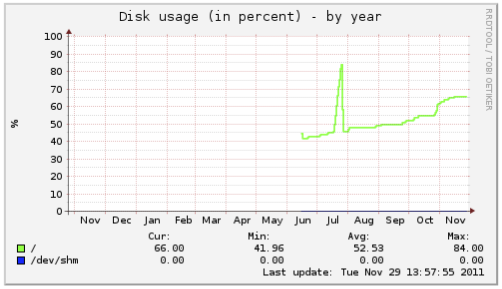
\includegraphics[width=\linewidth, keepaspectratio = true]{media/disk-usage-by-year.png}
\mycaption{figure}{\label{abb:disk-usage-by-year}Verhältnis von Speicheplatzverbrauch zur Speicherkapazität in Prozent in einer Zeitspanne von einen Jahr}
\end{center}

\subsection{Zugriffswachstum}
Für die Ist-Aufnahme konnten keine historischen Messdaten zur Verfügung gestellt werden.

\subsection{Skalierbarkeit Datenvolumen}
Während dem Betrieb ist ein Ausbau der Speicherkapazität (Skalierbarkeit) nicht möglich. Eine Vergrösserung der Speicherkapazität ist nur durch einen Wechsel auf ein anderes Hostingprodukt möglich. Dies erfordert eine Migration auf eine neue Server-Plattform. 

\subsection{Skalierbarkeit Datenzugriffe}
Keine Skalierbarung möglich. 

\subsection{Daten Durchsatz I/O}
Für die Ist-Aufnahme konnten keine Messdaten zur Verfügung gestellt werden.

\subsection{Daten Redundanz}

Die Daten-Redundanz wird durch das RAID-5 gewährleistet.

\subsection{Datenverfügbarkeit}
Stromausfälle und Netzwerkstörungen im Rechenzentrum des Hosting Providers führten zu Störungen und Ausfällen in der Webapplikation und in der Datenauslieferung. Die Störungen wurden jedoch nicht dokumentiert, weshalb keine statistische messbare Aussage über die erreichte Datenverfügbarkeit gemacht werden kann.

\subsection{Daten Sicherheit}
Die Daten sind durch physischen Fremdzugriff mittels Verschlüsselung geschützt. Für die Verschlüsselung wird das Device Mapper Module dm-crypt eingesetzt. dm-crypt verschlüsselt die Daten bereits auf Blockebene und ist somit für das Dateisystem tranRAID-5nt.

\subsection{Daten Integrität}
Zu jedem Bild wird eine Hash Prüfsumme gespeichert, die bei jedem Sicherung geprüft wird. Die Daten-Integrität ist somit sichergestellt.

\subsection{Sicherung}
Es wird täglich mittels dem Tool ccollect\footnote{\url{http://www.nico.schottelius.org/software/ccollect/}} ein R-Sync Sicherung der Daten erstellt. Das Sicherung wird ausser Hause gelagert.

\subsection{Wirtschaftlichkeit}
Die Kosten für die Speicherung der Daten inklusive Webinfrastruktur sind vergleichsweise zu alternativen Lösungen tief.

\subsection{Lokalität}

Die Web-Applikation inklusive dessen \gls{Primären-Daten} werden am selben Standort betrieben. Die Sicherungsdaten werden an einen seperaten Standort gelagert. Der Zugriff auf Sicherungs-Daten ist innerhalb 30 Minuten möglich.

\section{Analyse-Ergebnisse}

\subsection{System-Architektur}

\subsection{Datenwachstum und Speicherkapazität}
Die Messdaten aus dem  \refabb{abb:disk-usage-by-year} zeigen, dass das Datenvolumen seit  Juni 2011 bis Ende November 2011 mit Ausnahme einer unregelmässigen Spitze und einem grösseren Wachstumsschub Ende Oktober kontinuierlich zugenommen hat. Die etwas erhöhte Spitze lässt sich durch eine vorübergehende technische Änderung am System erklären und hat somit für die Auswertung keine Relevanz. Während der erwähnten Zeitspanne hat das Datenvolumen von 1,634 Terabyte auf 2,546 Terabyte zugenommen. Dies entspricht einer Datenzuwachsrate von 0,912 Terabyte bzw. 55,8\% in fünf Monate. Das Durchschnittliche Datenwachstum beträgt 0,182 Terabyte bzw. 11,1\% pro Monat.

Setzt sich der bisherige Trend fort, so ist die verfügbare Speicherkapazität von 3,8 Terabyte in weniger als 7 Monate erschöpft. Berücksichtigt man bei diesem durchschnittlichen Datenwachstum mögliche Wachstumsschübe für Neukunden, welche durch das Einlesen von deren bestehende Bilddatenbanken entstehen könnten, so reduziert sich die Kapazitätsreserve nach unten und würde eine vorzeitige Umstellung auf ein neues System bedingen.

Gemäss des Auftraggebers ist ferner ein neues Feature für die Web-Applikation geplant, welches den Speicherplatzbedarf verdoppeln würde. Die aktuelle Speichersituation lässt momentan den produktiven Einsatz des neuen Feature nicht zu. Das durchschnittliche Datenwachstum würde voraussichtlich auf 0,364 Terabyte pro Monat steigen.

Die jetzige Speicherkapazität erfüllt schon heute die Anforderungen nicht mehr.

\begin{equation}
\mbox{Datenwachstum}_{Monate5} = 2,546  \mathrm{TB} - 1,634 \mathrm{TB} =  0,912 \mathrm{TB}
\label{eqn:Verfügbarkeit_5Monate}
\end{equation}

\begin{equation}
\mbox{Datenwachstum}_{Monate5} = \frac{0,912 \mathrm{TB}}{\frac{1,634 \mathrm{TB}}{100 \%}} =  55,813\%
\label{eqn:Verfügbarkeit_5Monate_in_Prozent}
\end{equation}

\begin{equation}
\mbox{Durchschnittliches Datenwachstum}_{Monate} = \frac{0,912 \mathrm{TB}}{5\mathrm{m}} =  0,1824 \mathrm{TB}
\label{eqn:Verfügbarkeit_1Monate}
\end{equation}

\begin{equation}
\mbox{Durchschnittliches Datenwachstum}_{Monate} = \frac{55,813\%}{5 \mathrm{m}} = 11,162\%
\label{eqn:Verfügbarkeit_1Monate_in_Prozent}
\end{equation}

\subsection{Skalierbarkeit Datenvolumen}\label{AnalyseSkalierbarkeitDatenvolumen}
Die Eingesetzte Speicherarchitektur lässt eine Skalierung des Datenvolumen mittels hinzufügen von weiteren Festplatten oder durch Migration auf grösseren Festplatten zu. Die maximale Anzahl von Festplatten wird dabei durch die Anzahl vorhandenen SATA Anschlüsse im Server bestimmt. Beim eingesetzten Server handelt sich um eine Hosting Produkt welche meist begrenzt ausbaubar ist. Bei Hosting Produkte erfolgt eine Skalierung meist durch eine Wechsel auf eine besser ausgebautes Hosting Produkt. 

\subsection{Skalierbarkeit Datenzugriffe}
Eine mögliche Skalierung bezüglich des Datendurchsatzes könnte durch schnellere Festplatten, durch eine optimierte Verteilung der I/O-Operationen auf verschiedene Festplatten oder durch die Verteilung der Daten auf weitere Systeme erreicht werden. Zu beachten sind auch hier dieselben Prämissen, wonach wie beim Ausbau des Datenvolumens das bestehende System nur sehr begrenzt ausgebaut werden kann bzw. auf ein anderes Hostingprodukt migriert werden müsste.

\textbf{Skalierung durch schnellere Festplatten:}
Moderne Festplatten, mit Ausnahme von den teuren Solid State Disk (SSD), bieten zwar eine grössere Speicherdichte aber aufgrund der erreichten physikalischen Grenzen keine bedeutend effizientere IOPS versprechen. Eine Festplatte mit 7200 RPM erreicht durchschnittlich ein IOPS zwischen 75 und 100 IOPS. Bei SSD Disks wurden schon 1'190'000 IOPS in einem einzelnen PCI Geräte gemessen.\cite{Symantec2011} \cite{Fusionio} 
Ein Wechsel auf die genannten SSD Festplatten, ist aktuell noch mit sehr hohen Kosten pro Gigabyte verbunden. Gartner geht davon aus, dass 2012 die Preise pro Gigabyte bei SSD auf durchschnittliche 1\$ sinken werden. Gegenüber den heutigen Preisen bei konventionellen Festplatten von 30 Cents pro Gigabyte ist dies immerhin 3x teurer. Aus diesem Grund werden SSD Disks bei grossen Datenvolumen meist noch nicht eingesetzt, ausser spezielle Anforderungen an die Performance rechtfertigen die höhere Investition. \cite{AgamShah2011}

\textbf{Skalierung duch Verteilung der I/O Operationen:}
Ein RAID oder Volume Manager bietet die Möglichkeit, die I/O Operationen auf mehrere Festplatten zu verteilen. In einem RAID-5 verkleinert sich wie in Kapitel \refchap{AnalyseSkalierbarkeitDatenvolumen} beschrieben, die MTTF mit jeder weiteren Festplatte. Zudem sind die verfügbaren Anschlüsse in einem Server ebenfall ein zu berücksichtigen limitierender Faktor.

\textbf{Skalierung durch Verteilung der Daten:}
Nicht alle Kategorien von Daten haben die gleichen Anforderungen an den Durchsatz. Datenbanken z.B. benötigen in der Regeln einen höheren IOPS als statische Daten wie z.B. Bild-Daten, welche weniger oft abgefragt werden. Für die Verteilung der Daten ist eine Änderung in der System-Architektur und allenfalls in der Anwendungs-Architektur notwendig. Ein Beispiel für eine solche Anpassung der System-Architektur wäre die Auslagerung der Datenbank auf ein separates System, welches mit schnellen Solid State Disk ausgerüstet ist. 

\subsection{Redundanz}
Eine RAID-5 System bietet wie im \refsec{RAID-5} beschrieben, keine 1:1 Redundanz. Die Daten sind im RAID-5 nicht doppelt gespeichert, sondern werden bei einen Datenverlust mittels XOR Operation aus den Parität Stripes und den vorhandenen Daten Stripe-Einheiten berechnet. 

Bei einen Zugriff auf einen verlorenen Daten Stripe werden die Daten online berechnet. 

Treten bei einer Festplatte Fehler auf, werden die verlorenen Daten bei einem Zugriff aus dem Parität Stripe Einheit.??? Der Zugriff auf die Daten ist durch die Berechnung der Daten aus dem Parität Stripe Einheit Online möglich. Wird die ausgefallen Festplatte durch eine neu intakte Festplatte ersetzt, können die Daten durch einen Rebuild während des Betriebs wieder hergestellt werden. Durch die Berechnung und Schreib/Lese Operationen im RAID während des Wiederherstellungprozesses verschlechtert sich der Datendurchsatz und I/O Rate für den Datenzugriff wesentlich.

Einen Ausfall einer weiteren Festplatten kann das RAID-5 System nicht mehr kompensieren und führt zu einem physischen Datenverlust aller Online-Daten. Die Daten müssen in der Folge mittels des Sicherung eingelesen und wiederhergestellt werden, was jedoch nur im Offline-Betrieb möglich ist. 

Bei Festplatten welchen aus dem gleichen Produktionszyklus stammen, kann die Wahrscheinlichkeit eines weiteren Ausfall höher sein, im vergleich zu Festplatten die aus unterschiedlichen Produktionszyklen stammen.

\subsection{Service- und Daten-Verfügbarkeit}
Die bisherige System-Architektur gemäss dem Ist-Bestand ermöglichen keine AEC-2 Hochverfügbarkeit. Grund dafür ist die Fokussierung auf einen einzelnen Server in der System-Architektur. Der Server stellt eine "'Single Point of Failure"' (SPOF) dar. Tritt beim Server eine Störung auf, wie Sie zum Beispiel Aufgrund eines Gerätedefekts oder Softwarefehler auftreten können, kann der Service nicht von einem redundantem System übernommen oder weitergeführt werden. Eine Störung kann also die Verfügbarkeit während den Betriebszeiten starl gefährden und entspricht nicht den heutigen Anforderungen.

Die Netzwerkverfügbarkeit wird vom Hosting Anbieter gemäss den Allgemeinen Geschäftsbedingungen \cite{Ag2009} mit einer Verfügbarkeit von 99\% im Jahresmittel gewährleistet. Die Verfügbarkeit könnte somit bei einem 24x365 Stunden Betrieb während 87,6 Stunden nicht gewährleistet sein.

Das Speichersystem für sich selbst betrachtet kann die Verfügbarkeit und die Daten-Integrität gewährleisten, sofern keine Störungen durch einen Festplattendefekt eintreten. Das Speichersystem, welches ein interner Block-basierenden RAID-5 Speicher darstellt, ist ein Bestandteil des Serversystems und weist deshalb die selbe Verfügbarkeitsstufe wie das Serversystem auf. Die Service und Datenverfügbarkeit weist aus den genannten Gründen eine Verfügbarkeit Stufe von '"Highly Reliable"' AEC-2 auf.

Die im \refsec{System-Architektur}  beschriebene System-Architektur gewährleistet keine Hochverfügbarkeit der Daten. Einer der Gründe dafür ist, dass die Applikation nur auf einem einzelnen Server betrieben wird, dessen Hardware mit Ausnahme der Festplatten keine Redundanz aufweist und nicht für Hochverfügbar ausgelegt ist. 

Die Applikation wird auf einem einzelnen Server betrieben. Der Server und dessen Hardware mit Ausnahme der Festplatten stellen einen "'Single Point of Failure"' (SPOF) dar. Fällt der Server wegen eines Hardwaredefektes oder einem Softwarefehler aus, sind Daten und Anwendung für den Endbenutzer nicht mehr verfügbar.

Zudem werden die Daten und Applikation nur an einem Standort betrieben. Treten unvorhersehbare Ereignisse auf, wie z.B. ein lokaler Stromausfall, ein Brand oder eine Naturkatastrophe, kann der Betrieb nicht ohne die Wiederherstellung des ganzen Systems inklusive Daten von Sicherung wieder aufgenommen werden. Sofern nicht ein gemieteter Ersatzserver bereitsteht, muss ebenfalls die Beschaffung und Installation eines neuen Systems bei einem anderen Hosting Provider zur Ausfallzeit (Downtime) mit einberechnet werden. Der Service wäre während einer längeren Zeit nicht mehr verfügbar. Ein Kundenverlust und weitere Konsequenzen könnten die Folge sein.

\subsection{Daten Sicherheit}
Durch die Festplattenverschlüsselung sind die Daten bei abgeschaltetem Server vor unberechtigten Zugriffen geschützt. Befindet sich der Server jedoch im laufenden Betrieb, bietet die Verschlüsselung keinen Schutz vor Datendiebstahl. 

In einem Interview mit Ben Schwan im Technology Review hat Edward W. Felden, Professor für Informatik an der Princeton University den Grund dafür erklärt. 

\begin{quotation}\em
... ,die Dechiffrierungsschlüssel bei einer Festplattenverschlüsselung sitzen immer irgendwo im DRAM-Speicher. Um an sie heranzukommen, schaltet der Angreifer zunächst den Strom des Rechners aus und stellt die Energieversorgung dann gleich wieder her. Dann bootet er die Maschine in ein spezielles, böswilliges Betriebssystem hinein. Zu diesem Zeitpunkt enthält der Speicher noch immer die Originalinformationen, die verfügbar waren, als der Rechner noch nicht abgeschaltet wurde – die gewünschten Schlüssel natürlich auch. Das kurze Abschalten des Stroms hat daran rein gar nichts geändert. Der Angreifer kann dann die gewünschten Dechiffrierungsschlüssel aus dem Speicher auslesen und damit die geschützten Informationen auf der Festplatte jederzeit entschlüsseln\end{quotation}\cite{Schwan2008}

Des weiteren bietet eine Festplatten keinen Schutz bei Schwachstellen in der Software oder  der Konfiguration im laufenden Betrieb. Grund dafür ist, dass das Betriebsystem und Anwendungen über eine Verschlüsselungsschicht unverschlüsselt zugreifbar sind.


%!TEX root=../documentation-bachlorthesis-speicherarchitektur-lstucker.tex

\cleardoublepage
\chapter{Soll-Analyse}
Ziel ist es mit der Sollanalyse, den soll zustand Stand der System bzw. Speicherinfrastruktur, welche die verschiedenen Szenerien der Datenzuwachs und Datenzugriffe in den nächsten drei Jahren erfüllen soll  zu beschreiben. Der Auftraggeber geht von einen Starken Wachstum im Bereichen der Datenmengen und Datenzugriffe aus welche das Szenario 4 am ehesten wieder spiegelt.


\section{Szenario 1 - Schwaches Datenvolumen und Datenzugriff Wachstum}
Dieses Szenario beschreib den Soll-Zustand, wenn sich das Datenwachstum und Datenzugriffs Wachstum im gleichen umfang wie in der Ist-Analyse weiter entwickelt. Dieses Szenario würde eintreffen, wenn sich die Kunden Anzahlt und die gewünschten Aufbereitung der Daten für den Druck in den nächsten drei Jahre auf dem selben aktuellen Niveau befinden.


Datenwachstum in Prozent pro Monat: 5\% 

Datenwachstum in Tebibyte pro Monat: 0.19 Tebibyte

Speichervolumen in 36 Monaten: 9.34 Tebibyte

\subsection{Skalierbarkeit Datenzugriff}
Die bestehende Speicherarchitektur konnte die bisherigen Datenzugriff mit einen Web-Server zufriedenstellend erfüllen. Eine Skalierung der Zugriffe von mehreren Server soll deshalb nicht als Hauptkriterium sein sondern.

\subsection{Skalierbarkeit der Speicherkapazität}
Die Speicherkapazität soll exklusive der Datenredundanz bis mindestens 13 Tebibyte skalieren.

\subsection{Redundanz}
Dem Kunden wird einen Qualität Standard gewährleistet, die Original gespeicherten Daten, sollen vor Veränderung geschützt werden, aus diesen Grund soll die Daten Integrität beim Zugriff auf die Original Daten sichergestellt sein.



\subsection{Verfügbarkeit}
Die Verfügbarkeit soll mindestens dem AEC-2 Standard von Harvard Research entsprechen.

\subsection{Daten Integrität}
Dem Kunden wird einen Qualität Standard gewährleistet, die Original gespeicherten Daten, sollen vor Veränderung geschützt werden, aus diesen Grund soll die Daten Integrität beim Zugriff auf die Original Daten sichergestellt sein.

\subsection{Lokalität}
Die Daten sollen in einer minimal Version an einen weiteren Standort als Backup gehalten werden.



\section{Szenario 2 - Schwaches Wachstum Daten / mittleres Wachstum der Abfragen}
Dieses Szenario beschreib den Soll-Zustand, wenn sich das Datenwachstum im gleichen umfang wie in der Ist-Analyse weiter entwickelt, sich jedoch der Datenzugriff im vergleich zur Ist-Analyse stark steigert. Diese Szenario würde eintreffen, wenn sich die Kunden Anzahl in den nächsten drei Jahren auf dem gleichen Niveau hält, jedoch die Aufbereitung der Daten für den Druck stark zunimmt.

Datenwachstum in Prozent pro Monat: 5\% 

Datenwachstum in Tebibyte pro Monat: 0.19 Tebibyte

Speichervolumen in 36 Monaten: 9.34 Tebibyte

\subsection{Skalierbarkeit Datenzugriff}
Der Datenzugriff soll von mehreren Webserver welche die Bilddaten am Kunden ausliefern und Server welche die Original Bilder in das gewünschte Format umrechnen möglich sein. Die Anzahl Datenzugriffe soll von bis zu zwanzig Server möglich.

\subsection{Skalierbarkeit der Speicherkapazität}
Die Speicherkapazität soll exklusive der Datenredundanz bis mindestens 13 Tebibyte skalieren.

\subsection{Redundanz}
Die Daten sollen mindestens doppelt Redundanz haben.

\subsection{Verfügbarkeit}
Die Verfügbarkeit soll dem AEC-2 Standard von Harvard Research entsprechen.

\subsection{Daten Integrität}
Dem Kunden wird einen Qualität Standard gewährleistet, die Original gespeicherten Daten, sollen vor Veränderung geschützt werden, aus diesen Grund soll die Daten Integriät beim Zugriff auf die Original Daten sichergestellt sein.

\subsection{Lokalität}
Die Daten sollen in einer minimal Version an einen weiteren Standort als Backup gehalten werden.

\section{Szenario 3 - Starkes Wachstum Daten / schwaches Wachstum der Abfragen}
Dieses Szenario beschreib den Soll-Zustand, wenn sich das Datenwachstum im vergleich zum Ist-Zustand stark steigert, aber der Datenzugriff auf gleichen Niveau hält wie in der Ist-Analyse hält. Dieses Szenario würde eintreffen, wenn sich die Kunden Anzahl oder die Anzahl Bilddaten pro Kund stark steigert, jedoch die Aufbereitung der Daten für den Druck gleich bleiben würde.

Datenwachstum in Prozent pro Monat: 

Datenwachstum in Tebibyte pro Monat: 6 Tebibyte

Speichervolumen in 36 Monaten: 218,5 Tebibyte

Bilder mit einer Speichervolumen von 1 Gigibyte: 221'184

\subsection{Datenzugriff}
Durch den Geringen Zugriff auf die Daten, muss auf die Daten nicht parallel von vielen Systemen zugegriffen werden können.

\subsection{Redundanz}
Die Daten sollen in doppelte oder dreifacher Redundanz gespeichert werden.

\subsection{Speicherkapazität}
Es soll 300 Tebibyte an Speicherkapazität zur Verfügung stehen.

\subsection{Verfügbarkeit}
Die Verfügbarkeit soll dem AEC-2 Standard von Harvard Research entsprechen.

\subsection{Daten Integrität}
Dem Kunden wird einen Qualität Standard gewährleistet, die Original gespeicherten Daten, sollen vor Veränderung geschützt werden, aus diesen Grund soll die Daten Integriät beim Zugriff auf die Original Daten sichergestellt sein.

\subsection{Lokalität}
Die Daten sollen in einer minimal Version an einen weiteren Standort als Backup gehalten werden.

\section{Szenario 4 - Starkes Wachstum Daten / starkes Wachstum der Abfragen}
Dieses Szenario beschreib den Soll-Zustand, wenn sich das Datenwachstum und den Datenzugriff im vergleich zum Ist-Zustand stark steigert. Dieses Szenario würde eintreffen, wenn sich die Kunden Anzahl oder die Anzahl Bilddaten pro Kund stark steigert und somit auch die Anfragen zur Aufbereitung der Daten für den Druck.

Datenwachstum in Prozent pro Monat: 

Datenwachstum in Tebibyte pro Monat: 6 Tebibyte

Speichervolumen in 36 Monaten: 218,5 Tebibyte

Bilder mit einer Speichervolumen von 1 Gigibyte: 221'184

\subsection{Datenzugriff}
Auf die Daten müssen von verschiedenen Systemen gleichzeitig zugegriffen werden können.

\subsection{Redundanz}
Dem Kunden wird die Datensicherheit gewährleistet, aus diesen Grund sollen die Daten mindestens in doppelter oder dreifacher echter Redundanz gehalten werden.  Eine Redundanz durch Berechnung der Daten erfüllt diese Anforderung nicht sondern wird nur als Ergänzung für die Verfügbarkeit angesehen.

\subsection{Speicherkapazität}
Es soll 300 Tebibyte an Speicherkapazität zur Verfügung stehen.

\subsection{Verfügbarkeit}
Die Verfügbarkeit soll dem AEC-4 Standard von Harvard Research entsprechen. Bei hoher Kundenzahl und Speichervolumen, würde einen Unterbruch bei der Verfügbarkeit des Dienstes zu einen Repräsentation Schaden verursachen und Unsicherheit der Zuverlässigkeit bei den bestehenden Kunden in Bezug Ihrer Daten Verusachen.

\subsection{Daten Integrität}
Dem Kunden wird einen Qualität Standard gewährleistet, die Original gespeicherten Daten, sollen vor Veränderung geschützt werden, aus diesen Grund soll die Daten Integrität beim Zugriff auf die Original Daten sichergestellt sein.

\subsection{Lokalität}
Um eine Verfügbarkeit gemäss AEC-4 zu gewährleisten sollen die Daten Online über zwei Standorte zugreifbar sein. Eine Backup der Daten könnte an einen weiteren dritten Standort erfolgen.
%!TEX root=../documentation-bachlorthesis-speicherarchitektur-lstucker.tex
\cleardoublepage
\chapter{Speicherarchitekturen}

Sowohl private Personen als auch Unternehmen haben unterschiedliche Anforderungen an die Speicherung ihrer Daten. Während früher die Daten in der Regel in einem integrierten Speicher des Computersystems verwaltet wurden, werden heute eine breite Paletten an Speicherlösungen am Markt angeboten. Ein Grund dafür ist der kontinuierlich wachsende Bedarf an mehr Speicherkapazität aber auch zusätzliche Anforderungen an die Verwaltung der Daten, die Datensicherung. Spezifische Daten zu suchen und zu bearbeiten soll heute einfach, effizient und zu günstigen Kosten möglich sein, was laufend neue Lösungsansätze bedingt und es nicht einfacher macht, auf das richtige Pferd bzw. Technologie zu setzen. Wer möchte morgen schon gezwungen sein, seine mühsam aufbereiteten Daten in einem aufwendigen Migrationsverfahren, womöglich mit einem notwendigen Datenverlust, in ein neues System zu übernehmen? Eine genauere Betrachtung des Angebotsmarktes für die vorhandenen und die künftigen sich durchzusetzenden Technologien drängt sich deshalb auf.

Die heutigen am Markt erhältlichen Speicherarchitekturen lassen sich in der obersten Kategorie in Block- (Block-based), Datei- (File-based) und Objekt- (Object-based) basierte adressierende Systeme unterteilen. Die Kategorien zur Einteilung der verschiedenen Lösungen lässt sich nicht exakt zuordnen, da einige Speicherlösungen aus einem Mix aus mehreren Kategorien bestehenden können.

\section{Block-basierend}
Die Block-basierende Speicherarchitektur ist wohl die traditionellste von allen und ist die am weitverbreiteste Form. Die meisten Computersysteme, sei es Server, Desktop-PCs, Tablet-PC, Smartphones, Spielkonsole, verwaltet ihre Daten in einem blockbasierenden Speicher. Als Speichermedium wird in diesen Geräten oft eine magnetische Festplatte, Solid State Disk oder ein Flash-Speicher verwendet.

Bei Block-Speicher werden Daten in Blöcke gelesen und gespeichert (adressiert), ein Block bildet sich aus einer Sequenz von Bits bzw. Bytes. Die Grösse eines Blocks wird als Blocklänge bezeichnet und ist bei allen Blöcken einer Einheit gleich gross. 

Experten wie Mike Mesnier, Greg Ganger und Erik Riedel, sehen jedoch bei zunehmender Speichergrösse und Komplexität von Systemen fundamentale Einschränkungen von Block-Schnittstellen.

\begin{quotation}
\em Since the first disk drive in 1956, disks have grown by over six orders of magnitude in density and over four orders in performance, yet the storage interface (i.e., blocks) has remained largely unchanged. Although the stability of the block-based interfaces of SCSI and ATA/IDE has benefited systems, it is now becoming a limiting factor for many storage architectures. As storage infrastructures increase in both, size and complexity, the functions that system designers want to perform are fundamentally limited by the block interface. \end{quotation}\cite{Mesnier2003}

Vergleicht man die Performance der ersten Festplatte, welche von IBM produziert wurde, mit einer heute erhältlichen Seagate Festplatte (Jahr 2011), so hat sich die Speicherdichte von 2000 bit per Quadratzoll auf 625 Gigabyte und die Transferrate von 8 Kilobyte auf 600 Megabyte pro Sekunde verbessert. \cite{Seagate2011}\cite{Seagate2011a}

Für den Zugriff auf blockbasierende Speichersysteme werden meist Schnittstellen-Protokolle wie das Small Computer System Interface (SCSI) oder Advanced Technology Attachment (\gls{ATA}) verwendet. Diese Protokolle wurden jedoch in einer Zeit entwickelt, als man davon ausging, dass ein Blockspeicher jeweils nur von einem Computersystem verwendet wird und nicht mit mehreren Computersystemen geteilt werden soll. Diese Annahme für single user systems stimmt für den Consumer Elektronic Bereich mehrheitlich noch heute. In Bereichen jedoch, in denen grosse Speicherkapazitäten oder eine hohe Verfügbarkeit für viele gleichzeitige Benutzer gefordert sind, wie dies viele Geschäftsanwendungen charakterisiert, stimmen diese Annahmen nicht mehr.

Für blockbasierende Speicher, welche nicht als Server-interne Speicher bestehen, unterscheidet man den Direct Attached Storage (DAS) und das Storage Area Network (SAN). 

\subsection{Direct Attached Storage}
Bei DAS handelt es sich, wie es aus der englischen Bezeichnung zu entnehmen ist, um Speicher, welcher direkt an ein Computersystem angeschlossen wird. Bei DAS Enclosure handelt sich um ein Gehäuse mit mehreren verbauten Festplatten, welche üblicherweise über einen Host-Bus-Adapter an ein Computersytem angeschlossen werden. Als Schnittstellen-Protokoll werden \gls{ATA}, \gls{SATA}, \gls{eSATA}, \gls{SCSI}, \gls{SAS} oder Fibre Channel eingesetzt. DAS können mit mehreren Computersystemen geteilt werden, sofern genügend Schnittstellen zur Verfügung stehen.

\subsection{Storage Area Network}
Die Storage Networking Industry Association (\gls{SNIA}) definiert ein Storage Area Network (SAN) als ein Netzwerk, dessen primärer Bestimmungszweck das Transferieren von Daten zwischen Computersysteme und Speicherelemente und unter Storage Elemente ist. Ein SAN besteht aus einer Kommunikations-Infrastruktur, welches eine physische Verbindung und eine Management-Schicht beinhaltet, das die Verbindungen, die Speichereinheiten und das Computersystem organisiert, damit der Datentransfer sicher und robust erfolgen kann. Der Begriff SAN wird normalerweise (aber nicht notwendigerweise) mit dem Block I/O Service in Verbindung gebracht und weniger mit dem Datei-Zugriff-Service. \cite{SNIA2011}

Je nach SAN Implementierung kommen folgende Geräte bzw. Komponenten vor:
\begin{itemize}
\item Server
\item Host Bus Adapter
\item Gigabit Interface Converter
\item SAN-Switch
\item Storage system (Speichersystem)
\item Tape Library
\item Logical Unit
\end{itemize}

\paragraph*{Server} 
Der Server greift über das SAN auf Ressourcen von Speichersystem oder Tape Library zu. In einzelnen Fällen kann der Server selbst über SAN anderen Servern Speicher zur Verfügung stellen.

\paragraph*{Host Bus Adapter}
Host Bus Adapter (HBA) für das SAN sind intelligente Hardwareschnittstellen, welche für die Verbindung von Server in einem SAN verwendet werden. Sofern die Server nicht bereits mit einem Host Bus Adapter ausgerüstet sind, können diese normalerweise durch Host Bus Adapter in form von Steckkarten erweitert werden. Der Host Bus Adapter selber hat pro Port einen Einschub, in welche ein Gigabit Interface Converter eingebaut wird. \cite{Christopher2009}

\paragraph*{Gigabit Interface Converter}
Der Gigabit Interface Converter ist eine modulare Schnittstelle, welche elektrische Signale in optische Signale umwandeln. \cite{SNIA2011}

\paragraph*{SAN-Switch}
Der SAN Switch ist ein Koppler, welcher dezidiert für die SAN-Umgebung verwendet wird.

\paragraph*{Speichersystem}
Das Speichersystem stellt im SAN den geteilten Speicher zur Verfügung. Gemäss den IT Marktforschung und Analyse Unternehmen Gartner gehören \gls{EMC}, \gls{IBM}, NetApp, \gls{Dell}, \gls{HP}, \gls{HitachiDataSystems} zu den Marktführern. \cite{RogerW.CoxPushanRinnenStanleyZaffos2011}

\paragraph*{Tape Library}
Tape Library ist eine Bandbibliothek, in welchem sich ein oder mehrere Bandlaufwerke und mehrere Magnetbänder befinden und meistens der automatische Bandwechsel mittels eines Bandroboters realisiert wird. Das Tape Library wird für die Sicherung von Daten auf Band eingesetzt.

\paragraph*{Logical Unit}
Ein Logical Unit ist ein Gerät, welches über SCSI-Protokoll über das Logical Unit Number (LUN) andressiert wird. Das Gerät wird, technisch nicht korrekt, oft als LUN bezeichnet. Im Speichersystem werden z.B. mehrere Festplatten mittels RAID zu einer Einheit zusammengefasst. Sofern keine weitere Virtualisierung von dem Speicherhersteller zum Einsatz kommt, wird die zusammengefasste Einheit wiederum in Speichereinheiten aufgeteilt und diese als LUN dem Server zugeteilt. \cite{SNIA2011}

\subsubsection{Fibre Channel}
SCSI ist zwar sehr populär, ist jedoch mit 80 Mbps Geschwindigkeit, mit maximal 25 Meter Buslänge und mit maximal 32 Geräten pro Bus, ein limitierender Faktor für viele Anwendungen. Unter anderem wegen den erwähnten Limitierungen von SCSI hat das American National Standards Institute (ANSI) die Fibre Channel Technik entwickelt. Fibre Channel ist ein mehrschichtiges Netzwerk, welches die charakteristischen Funktionen für die Übertragung von Daten über ein Netzwerk definiert. Der Standard enthält von der physikalischen Schnittstelle, Daten Codierung, Übertragungssteuerung (Link Control), Fluss Kontrolle, bis hinzu den Protokoll Schnittstellen. Im Vergleich zu anderen Netzwerken beinhaltet die Fibre Channel Architektur einen signifikanten Anteil von Hardware Prozessen, um eine hohe Performance zu erreichen. \cite{Gupta2002}\cite{Christopher2009}

Beim Design von Fibre Channel hat man darauf geachtet, die besten charakteristischen Eigenschaften der I/O Bus-Kommunikation (Channel) zwischen zwei Geräten und der Netzwerk- Kommunikation zwischen mehreren Geräten zu kombinieren. Die Channel-Kommunikation ist im Vergleich zur Netzwerk-Kommunikation, hardwareintensive, schnell und produziert wenig Overhead. Netzwerk-Kommunikation ist hingegen abhängig von der Softwareimplementierung, das Protokoll, unterstützt aber die Kommunikation für eine grosse Anzahl von Geräten.

Anders als es der Namen von Fibre-Channel vermuten lässt, ist Fibre-Channel nicht auf Fiberoptik-Kabel als Träger-Medium beschränkt, sondern lässt sich ebenso mit Kupferkabel betreiben. Aufgrund von physikalischen Eigenschaften ist das Fiberoptik-Kabel gegenüber dem Kupferkabel in Geschwindigkeit kombiniert mit Distanz überlegen. So liegt die maximale Distanz bei Kupferkabel bei 30 Metern bei einer Geschwindigkeit von 1 Gbps, bei höheren Geschwindigkeiten wird die maximale Distanz noch weiter reduziert. Beim Fiberoptic-Kabel wird die maximale Distanz der Signalübertragung von der Installationsqualität, des Fiberoptic-Kabeltyps, des Kern-Durchmessers, der Lichtwellenlänge Rundreise Latenz und der eingesetzter Hardware bestimmt. Je weiter das Licht innerhalb des Kabels übertragen werden muss, desto grösser ist der Verlust der ursprünglichen Signalstärke. Mit spezieller Hardware können auch Distanzen von bis zu 600 Kilometer \footnote{\url{http://www.enterprisestorageforum.com/industrynews/article.php/2171801/Synchronous-SAN-Sets-Fibre-Channel-Distance-Record.htm}} erreicht werden.

Es gibt drei Fibre Channel Topologien:
\begin{itemize}
\item Point-to-Point
\item Arbitrated-Loop
\item Switched-Fabric
\end{itemize}

\paragraph*{Point-to-Point-Topologie}
Die Point-to-Point-Topologie ist die direkte Verbindung von zwei Fibre Channel Geräten. Oft handelt es sich um eine Verbindung von einem Server und einem Speichersystem, wie dies im Direct Attached Storage (DAS) Umfeld vorkommt. \cite{Christopher2009}

\paragraph*{Arbitrated-Loop-Topologie}
Bei der Arbitrated-Loop-Topologie können bis zu 126 Knoten (NL\_Ports) in einem geteilten Bus-Ring zusammengeschlossen werden. In diesem Ring kann eine Verbindung zwischen zwei Ports aktiv sein, während alle anderen Ports als Repeater arbeiten und das Signal weiterleiten. Die Arbitrated-Loop-Topologie ist in seiner Architektur dem Token-Ring ähnlich. \cite{Gupta2002}\cite{Christopher2009}

\paragraph*{Switched-Fabric-Topologie}
Die klassische SAN Topologie basiert auf der Switched-Fabric-Topologie. Eine Switched-Fabric-Topologie besteht aus einer oder mehreren Switches, die zu einer Fibre-Channel-Fabric zusammengeschlossen werden. Die einzelnen involvierten FC-Geräte, wie Server oder Storagesysteme, werden über eine oder mehrere Ports an eine Switched-Fabric angeschlossen. In einer Fabric können bis zu $2^{24}$ Ports angeschlossen werden. \cite{Gupta2002}\cite{Christopher2009}

Mit der Switched-Fabic-Topologie lassen sich verschiedene Fabric Topologien bilden.
Die einfachste Topologie, welche die Eliminierung von "'Single Point of Failure"' zum Ziele hat, ist die Dual Switch Topologie, wie in der \refabb{abb:DualSwitchTopologie} dargestellt. In dieser Topologie dient jeder Switch als eigenständige Fabric. Die FC-Geräte wie Server und Storagesysteme werden jeweils pro Fabric bzw. Switch mit mindestens einem FC-Port angeschlossen. Durch den Einsatz von Path Management Software auf dem Server, kann eine vom Speichersystem zugeteilte Logical Unit über mehrere Path angesprochen werden. Diese Implementierung bietet gleich verschiedene Vorteile. Wenn ein Path oder eine ganze Fabric ausfallen sollte, übernimmt der andere Path automatisch die Kommunikation. Bei Wartungsarbeiten an Komponenten einer Fabric kann der Service ohne Downtime des Gesamtsystems weiter betrieben werden. Moderne Path Management Software und Speichersysteme unterstützen zudem die Lastverteilung (Loadbalance) der I/O-Last über alle Paths. \cite{Christopher2009}

\begin{center}
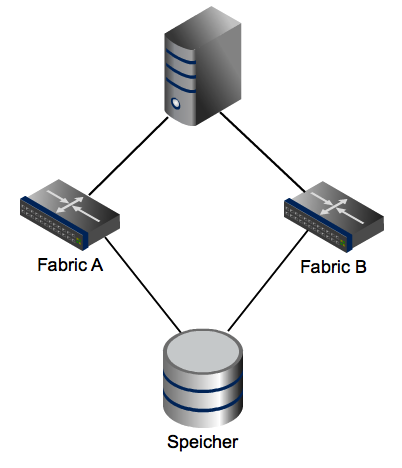
\includegraphics[width=\linewidth, keepaspectratio = true]{media/dualSwitchTopologie.png}
\mycaption{figure}{\label{abb:DualSwitchTopologie}Fibre Channel SAN mit Dual Switch Topologie}
\end{center}

Die Meshed Fabric Topologie erhöht die zusätzlich die Ausfallsicherheit innerhalb einer einzelnen Fabric. Für die Meshed Fabric sind pro Fabric mindestens vier Fibre Channel SAN Switches erforderlich. Jeder Switch wird, wie in \refabb{abb:MashedFabricTopologie} ersichtlich, mit mindestens einem Path, den sogenannten Inter-Switch-Link (ISL), zu allen anderen Switches in der Fabric verbunden. Die Meshed Fabric kann den gleichzeitigen Ausfall von mehreren Kabeln und Switches verkraften, ohne dass deshalb die ganze Fabric ausfällt. \cite{Christopher2009}

\begin{center}
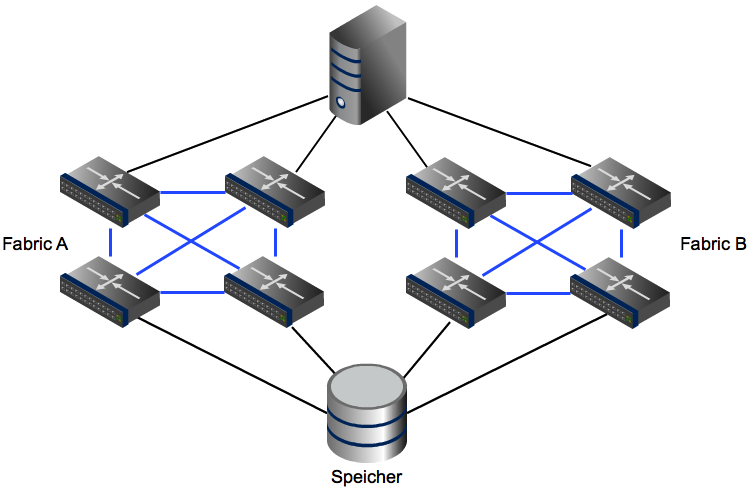
\includegraphics[width=\linewidth, keepaspectratio = true]{media/MashedFabric.png}
\mycaption{figure}{\label{abb:MashedFabricTopologie}Fibre Channel SAN mit Mashed Fabric Topologie}
\end{center}

\subsubsection{iSCSI}
Das SCSI-Protokoll ist ein populäres Protokoll für die Kommunikation mit I/O Geräten speziell für Speichergeräte. SCSI weist die Client-Server Architektur auf, wobei die Clients bei SCSI Interfaces als "initiators" bezeichnet werden und die logische Einheit vom Server als "target".

SCSI Protokoll wurde schon über Protokolle transportiert, jedoch waren all die Transportprotokolle in der Distanz limitiert. \gls{IBM} startete 1996 mit der Forschung für die Übertragung von SCSI über das Ethernet, dabei untersuchte \gls{IBM}, ob sich der Transport mittels IP oder \gls{TCPIP} besser eignen würde. Messungen zeigten damals, dass in einem lokalen Netzwerk der Transport mittels IP besser als \gls{TCPIP} geeignet ist. Mit den erwarteten künftigen Entwicklungen bezüglich des Datentransports über die lokalen Netzwerkgrenzen hinaus war hingegen der Einsatz von TCP/IP die bessere Wahl. 1999 hatten sich \gls{IBM} und \gls{Cisco} darauf geeinigt, "SCSI over TCP/IP" gemeinsam in einer Internet Engineering Task Force (\gls{IETF}) als Industriestandard weiterzuentwickeln \cite{JohnL.202}. Die definitive Spezifikation von SCSI over \gls{TCPIP} ist im \gls{RFC} 3720 mit dem Namen iSCSI im April 2004 fertiggestellt worden. \cite{J.Satran2004}

% \paragraph*{Kosten}
Für den Betrieb eines Fibre Channel SAN sind spezielle Hardware und Fibre Channel Kenntnisse notwenig. Da bei iSCSI dieselbe Technik wie im Computernetzwerk verwendet wird, benötigt der Aufbau und Betrieb von Netzwerk Infrastruktur und Management Software Lösungen keine zusätzliche Ausbildung, was die Gesamtbetriebskosten (TCO) substanziell senkt.

Grundsätzlich kann jeder Computer, welcher mit einem Netzwerkanschluss ausgerüstet ist und einen iSCSI Software Treiber hat, iSCSI nutzen. Computer, welche genügende Prozessorleistung aufweisen, können die zusätzliche Last für die Verarbeitung von iSCSI mit konventionellen Netzwerkkarten lösen. Computersysteme für welche die Verarbeitungsgeschwindigkeit kritisch ist, kann diese zusätzliche Last eine Bürde sein. Vergleichbar wie bei Fibre Channel gibt es für iSCSI spezielle Netzwerkkarten bzw. Host Bus Adapter, welche mittels TCP/IP Offload Engine (TOE) und volle iSCSI Offload Engine im eigenen Chip die \gls{TCPIP} bzw. iSCSI Pakete verarbeiten. Solche Netzwerkkarten entlasten die Central Processing Unit (\gls{CPU}) des Servers wesentlich und weisen bessere Werte in der Latenz auf.

% \paragraph*{Netzwerk}
In einem Ethernet Netzwerk verwaltet sich jeder Switch mehr oder weniger autonom und führt eine eigene Weiterleitungstabelle, mit welcher der Switch entscheidet, über welchen Port ein Ethernet Paket ausgeliefert werden muss. Dazu enthält die Weiterleitungstabelle pro MAC Adresse den dazugehörigen Port. Trifft ein Ethernet Paket mit noch unbekannter MAC Adresse ein, leitet der Switch das Paket über alle Ports weiter. Durch die Rückantwort vom Zielsystem lernt der Switch, über welchen Port dieses erreichbar ist. Werden in einem Switch Netzwerk benachbarte Switches untereinander über mehrere Pfade verbunden, kann es in einem solchen Szenario vorkommen, dass das Paket wieder am ursprünglichen Switch ankommt, wenn der benachbarte Switch die MAC-Adresse ebenfalls nicht kennt. Es entsteht dadurch eine Verdoppelung des Ethernet Paketes im Netzwerk bzw. es kommt zu einer Schleifenbildung, was in der Folge zu einer Netzwerkstörung führt. Mittels Spanning Tree Protokoll (STP) sollen solche Schleifen vermieden werden. Das Spanning Tree Protokoll erstellt eine Baum Topologie mit jeweils einem aktiven Path zwischen zwei Switches. Diese Topologie hat verschiedene Nachteile: 

\begin{itemize}
\item Beim Topologie-Wechsel wird im Netzwerk der Spanning Tree neu ausgehandelt. Während dieser Neuaushandlung ist der Datentransport während mindestens 15 Sekunden unterbrochen. Ein typischer Topologiewechsel kann zum Beispiel durch einen Pfad-Ausfall zwischen zwei Switches hervorgerufen werden.

\item In einer Baum-Hierarchie müssen die Pakete innerhalb des Baumes der Hierarchie entsprechend weitergeleitet werden (auf und ab) und können nicht über einen theoretisch direkteren Pfad quer weitergeleitet werden. Befindet sich z.B das Ziel auf der anderen Baumseite, muss das Paket die ganze Hierarchie hinauf und auf der anderen Seite hinunter bis zum Zielsystem weitergeleitet werden. Könnten die Switches über mehrere Pfade miteinander kommunizieren, so würde dem Datentransport über den direkten Weg nichts im Wege stehen und würde zudem weniger Switches involvieren bzw. belasten.
\end{itemize}

Hersteller wie Brocade haben diese Problematik für den Betrieb von iSCSI SAN erkannt und haben Lösungen entwickelt, welche das Prinzip von Fibre Channel Fabrics für Ethernet Netzwerke umsetzen. Bislang ist dafür noch kein allgemein verbindlicher Standard entstanden und proprietäre Lösungen sich im Markt kaum durchsetzen können.

%\paragraph*{Sicherheit}
Wie beim Fibre Channel SAN sollte im Geschäftsumfeld iSCSI über ein dediziertes Netzwerk laufen. Die Abgrenzung erhöht die Sicherheit einerseits und das Storage Netzwerk ist andererseits klar von anderen Netzwerken abgeschottet. Fehlerhafte Firewall-Regeln für das Computer Netzwerk haben keinen direkten Einfluss auf die Sicherheit des Datennetzwerkes. Störungen oder Überlast im Computer Netzwerk beeinflussen nicht die iSCSI Verbindungen. Mittels IPsec kann die Sicherheit durch die verbesserte Authentifizierung und der optionaler Verbindungsverschlüsselung weiter erhöht werden. 

%\paragraph*{Integrität}
iSCSI stellt die Integrität des übermittelten Paketes mit dem CRC-32c Digests sicher. 

\paragraph*{Skalierbarkeit Datenvolumen}
Einem Server können mehrere Logical Units zugeteilt werden. Durch den Einsatz eines Volume Managers können mehrere Logical Units zu einer grossen logischen Volume zusammengefasst werden. Sollte die Kapazität eines Speichersystems nicht ausreichen, kann ein weiteres Speichersystem an das SAN angeschlossen werden.

\paragraph*{Durchsatz I/O}
Die Firma Netapp zählt zu den Marktführern für unternehmensweite NAS Speicherlösungen. Neben dem "Network File System" (NFS), unterstützen die Speicherlösungen von Netapp auch die Integration von Logical Units über iSCSI als auch über Fibre Channel. Saad Jafri und Chris Lemmons von Netapp haben die Bereitstellung von Speichern über die verschiedenen Verfahren bezüglich Performance für eine VMWare vSphere Umgebung untersucht. Netapp weisst in ihrem Report nicht die konkreten Messwerte aus, sondern lediglich die Werte im Vergleich zu einem 4Gb Fibre Channel.

Wie im \refabb{abb:NetappIOPS} von Netapp zu entnehmen ist, sind die I/O pro Sekunden Werte von iSCSI in einen 1Gb Ethernet Netzwerk im Vergleich zu dem 4Gb Fibre Channel rund 8\%tiefer. Wobei höhere Werte bei I/0 pro Sekunden besser sind. Im 10 Gb Ethernet Netzwerk erreicht iSCSI dieselben Werte wie Fibre Channel in einem 8Gb Netzwerk. \cite{Jafri2011}

\begin{center}
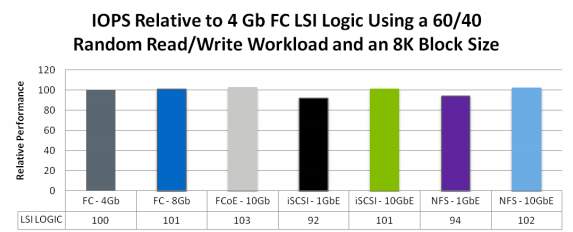
\includegraphics[width=\linewidth, keepaspectratio = true]{media/netapp_iops.png}
\mycaption{figure}{\label{abb:NetappIOPS}Netapp IOPS Durchsatz für alle unterstützten Protokolle im Vergleich zu 4Gb FC mit 8K Blockgrösse\cite{Jafri2011}}
\end{center}

Der Report von Netapp hat ebenfalls die Latenz verglichen. Bei der Latenz möchte man einen möglichst tiefen Wert erreichen. Gemäss \refabb{abb:NetappLatenz} ist die Latenz von iSCSI in einen 1 Gb Ethernet Netzwerk rund 9\% höher als bei Fibre Channel in einem 4Gb Netzwerk. Bei iSCSI in 10Gb Ethernet waren die Werte gleich gut wie Fibre Channel im 4Gb Netzwerk. Das Fibre Channel in einem 8Gb Netzwerk hatte jedoch rund 1\% tiefere Werte.\cite{Jafri2011}

\begin{center}
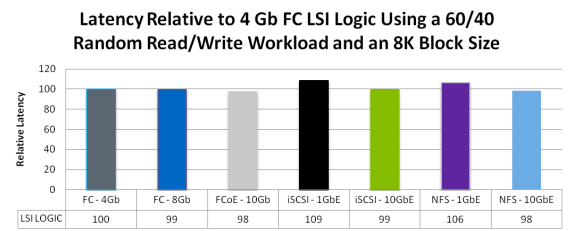
\includegraphics[width=\linewidth, keepaspectratio = true]{media/netapp_latence.png}
\mycaption{figure}{\label{abb:NetappLatenz}Netapp Latenz für alle unterstützten Protokolle im Vergleich zu 4Gb FC mit 8K Blockgrösse \cite{Jafri2011}}
\end{center}
 
\subsection{Logical Volume Manager}
Logical Volume Manager oder Dateisysteme, welche die Logik eines Logical Volume Managers kombinieren, ermöglichen mehrere Block-Geräte bzw. Logical Units zu einer grossen logischen Volume zusammenzufassen. Dies birgt den Vorteil, dass die maximale Grösse eines Block-Gerätes nicht der limitierende Faktor des darauf installierten Dateisystems ist. Neben dem Erstellen von Logischen Volumes können einige Logical Volume Manager den Last-Zugriff auf die verschiedenen Block-Geräte durch Striping optimaler verteilen und sorgen damit für eine besser Performance beim Datenzugriff. Eine weitere Aufgabe des Logical Volume Managers ist die redundante Haltung der Daten durch Spiegelung. Mittels serverseitiger Spiegelung (Host-Based Mirroring) können die Daten von zwei Standorten zur Verfügung gestellt werden. Dazu werden von zwei Speichersystemen, welche an unterschiedlichen Standorten installiert sind, gleich viele und gleich grosse Logical Units über das SAN dem Computersystem zugeteilt.

Klassische Server Linux Distributoren, wie Red Hat, Suse und Debian inkl. Ubuntu liefern den quelloffenen Logical Volume Manager 2 (LVM2) in ihrem Distributionspacket mit. Der LVM2 kann theoretisch auf einem 64-Bit System eine Logical Volume von 8 Exabyte bilden und adressieren. \cite{Levine2009}

Das ursprünglich von Oracle als ZFS-Ersatz entwickelte Btrfs Dateisystem könnte sich künftig zum Standard Dateisystem für viele Linux Server Distributionen mausern. Das für Solaris entwickelte ZFS als auch Btrfs kombinieren Dateisystem und Logical Volume Manager. Btrfs selbst wurde jedoch noch nicht als stabile Version veröffentlicht und ist deshalb für den produktiven Betrieb noch nicht empfehlenswert. \cite{Redler2011}


\subsection{Datei System}
Betriebssysteme adressieren die Daten auf Block-Geräten nicht direkt an, sondern greifen über das darüberliegende Dateisystem zu. Das Dateisystem organisiert wie und wo Dateien auf den Block-Geräten abgelegt werden und verwalten die freie Speicherkapazität. Einige Dateisysteme regeln auch die Zugriffsberechtigungen auf die Daten. Die Block-Geräte (Logical Units) können im SAN oder DAS an verschiedene Computersysteme gleichzeitig zugeteilt werden. Es ist die Aufgabe des Dateisystems sicherzustellen, dass mehrere Computersysteme gleichzeitig vom gleichen Dateisystem lesen bzw. auf dieses schreiben können. Konventionelle Dateisysteme wie Ext3 unter Linux gehen von einer exklusiven Nutzung des Speichers aus. Dieses Dateisystem enthält keine Funktionen, die den gleichzeitigen Zugriff auf Daten regeln. Problematik beim gleichzeitigen Zugriff ist die Sicherstellung der Datenkonsistenz. Schreiben zum Beispiel zwei Computersysteme gleichzeitig in dieselbe Datei, ist zu regeln, welche Änderung gültig ist, um Dateninkonsistenz zu vermeiden. Dateisysteme, welche den gleichzeitigen Datenzugriff erlauben, regeln den Zugriff auf Dateien z.B. mit einem Sperrmechanismus (locking). Schreibt ein Computersystem in eine solche gleichzeitig benutzte Datei, wird die Datei für Änderungen durch das andere Computersystemen gesperrt. Dieser muss sich den neuen aktuellen Stand mit einem Daten-Refresh wieder holen. Cluster Dateisysteme wie Red Hat Global Filesystem (GFS) und Red Hat Global Filesystem 2 (GFS2) unterstützen dieses Sperren. Das Dateisystem Red Hat GFS Version 2 unterstützt bei einem 64-bit-System theoretisch Dateisysteme bis 8 Exabyte, Red Hat gewährleistet jedoch nur einen Support von maximal 100 Terabyte. \cite{Levine2011}

Dateisysteme wie ZFS und Btrfs stellen die Integrität der Daten vor Veränderung, wie dies zum Beispiel durch einen Bit-Fehler auf dem Block Gerät oder im Memory entstehen könnte, mittels Prüfsumme sicher. Dabei wir zur jeder Datei eine Hash-Prüfsumme abgespeichert. Wird die Datei gelesen, wird die Prüfsumme aus der Datei neu berechnet und mit der abgespeicherten Prüfsumme verglichen. Sofern das Dateisystem ebenfalls gespiegelt ist, korrigiert das Dateisystem die fehlerhafte Datei aus der intakten Kopie automatisch. Dieses Verfahren wird auch als selbstheilend (self-healing) bezeichnet. \cite{Bonwick2005}\cite{Oracle}

Dateisysteme können mittels Sicherungssoftware auf Bandlaufwerke oder andere Speichermedien gesichert werden.


\section{Datei-Basierend}
Bei Datei-basierten Speicherarchitekturen werden Daten nicht wie bei Block-basierten Speicherarchitekturen über Blocke adressiert, sondern über Dateien.

Mit dem Aufkommen von Desktop-Computern, wurde die Rechenlast des zentralen Mainframecmputer wesentlich entlastet (verteilte Rechenlast auf viele kleine Rechner). Ohne die Vernetzung der Desktop-Computer mussten die Daten mittels portablen Speichermedien ausgetauscht werden. Dies mag in kleinen Umgebungen noch praktikabel gewesen zu sein, wurde jedoch mit der steigenden Anzahl der Teilnehmer zusehends schwieriger bis unmöglich. Verfügbarkeit und Konsistenz der Daten konnte nicht zufriedenstellend gelöst werden. Die direkte Vernetzung der Desktop-Computer erlaubte zwar den effizienten Datenaustausch über das Netzwerk, bot aber trotzdem keine gefällige Lösung für die Datenkonsistenz und Datensicherung. Die bessere Lösung war der gemeinsame zentral angelegte Speicher, in welchem sämtliche Unternehmensdaten für alle Benutzer verfügbar gehalten und mit einem regelmässigen Backup gesichert wurden. Alle Anwender verfügten immer über die aktuellste Version der Daten. Unternehmen wie Sun Microsystem, IBM, Microsoft und Apple erkannten die Bedürfnisse der Benutzer und entwickelten für ihre Betriebsysteme die Funktionen für den geteilten Datenzugriff.

Zu den bekanntesten und weitverbreitesten Lösungen zählen NFS und \gls{CIFS} (SMB).


\subsection{Network File System}
Das ursprünglich rein von der Firma SUN Microsystems (heute Oracle) 1984 entwickeltes Network-File-System, ermöglicht den gemeinsamen Zugriff von mehreren Computersystemen auf das Dateisystem eines zentralen Host (Server), als ob der einzelne Benutzer Zugriff auf ein lokales Dateisystem hat. Die zweite Version von NFS erschien 1989 und war die erste Version welche von Internet Standard Request for Comments (\gls{RFC}) standardisiert wurde und unter der \gls{RFC} Nummer 1094 \footnote{\url{http://tools.ietf.org/html/rfc1094}} veröffentlicht wurde. Für den Transport des NFS Protokolls wurde bis Version zwei ausschliesslich das \gls{UDP} Transportprotokoll unterstützt.
Die Version 3 von NFS (\gls{RFC} 1813)\footnote{\url{http://tools.ietf.org/html/rfc1813}}, die 1995 veröffentlicht wurde, war die erste Version, in der Computer, Betriebsystem, Netzwerk-Architektur und Transport-Protokoll unabhängig ist. Die Unabhängigkeit wird mit der Verwendung von Remote Procedure Call (\gls{RPC}) erreicht, welches wiederum ein eXternal Data Representation (\gls{XDR}) verwendet. \cite{Stern2001}

\begin{center}
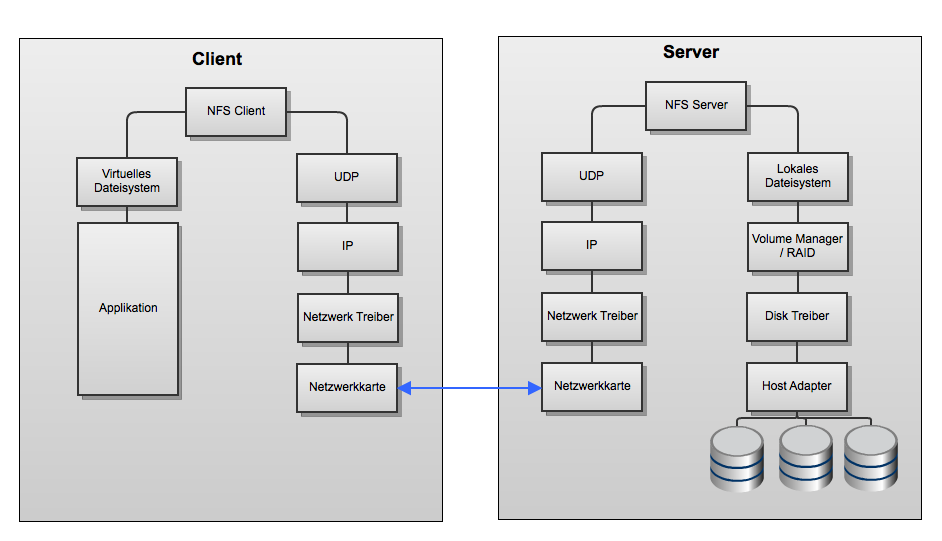
\includegraphics[width=\linewidth, keepaspectratio = true]{media/NFS.png}
\mycaption{figure}{\label{abb:NFSArchitektur}NFS Architektur \cite{Jafri2011}}
\end{center}

Wie im \refabb{abb:NFSArchitektur} zu entnehmen ist, ist NFS eine weitere Schicht, welche auf dem Dateisystem und dessen Block-Geräten des Computersystems bzw. Speichersystem aufbaut. So ist es zum Beispiel die Aufgabe des Dateisystems bzw. des Block-Gerätes, die Redundanz und Integrität der gespeicherten Daten sicherzustellen. 

Die Datenkonsistenz für den gleichzeitigen Zugriff von mehreren Computern stellt NFS mit einem separaten Protokoll, dem Network-Lock-Manager (NLM) sicher. Der Network-Lock-Manager sorgt dafür, dass eine Datei, welche von einem Computersystem geändert wird, vor der Änderung durch andere Benutzer, gesichert ist. Wenn ein Client eine Sperrung angefordert hat, muss derselbe Client dem Server die Entsperrung mitteilen, nachdem er die Daten nicht mehr benötigt. Diese Sperrlogik führt jedoch zu Problemen, wenn der Client vor der Entsperrung ein Systemabsturz erleidet, also die Entsperrung gar nicht mehr melden kann und somit die Datei für alle anderen Benutzer gesperrt bleibt.
NFS setzt mit NLM das Advisory Locking Sperr-Verfahren ein. Das bedeutet, dass andere Clients beim Zugriff auf eine gesperrte Datei nur darauf hingewiesen werden, dass die Datei gesperrt ist, ohne den Client daran zu hindern, eine gewünschte Änderung an den Daten vorzunehmen. \cite{Stern2001}

Seit Version 4 von NFS Protokoll (\gls{RFC} 3530) ist das Sperrverfahren (Locking) im Protokoll selber implementiert. Dadurch entfällt der zusätzliche Einsatz des Network Lock Managers. NFS Version 4 unterstützt zudem das Sperren eines Bytes-Bereiches innerhalb einer Datei. Der Client erhält vom Server lediglich einen Leasing-Zeitraum für die Sperrung (Lock), welche der Client vor Ablauf der Frist wieder erneuern muss, um sie aufrechtzuerhalten. NFS in der Version 4 erlaubt ferner das Sperrverfahren Mandatory Locking, das allen anderen Clients nicht ermöglicht, sich über die Sperrung hinwegzusetzen. \cite{Callaghan2003}

Indem NFS auf TCP/IP als Kommunikationsprotokoll aufbaut, kann eine NFS Freigabe, Standort übergreifend festgelegt werden. Es gilt auch hier, dass die Latenz und die Bandbreite der Verbindung zwischen den Standorten entscheidend ist und limitierend wirken kann.

NFS selbst hat keine eigene Implementierung für die Sicherstellung der Datenintegrität. Stattdessen verlässt sich NFS seit Version 2 auf die TCP und Ethernet Fehlererkennung. TCP prüft im Standardverfahren die Integrität mit einer 16-Bit-Integer Prüfsumme. Die 16-Bit-Integer Prüfsumme erkennt Fehler im pseudo IP-Header, TCP-Header und Daten. Das Verfahren zeigt Schwächen bei einzel Bit-Fehlererkennung. Ethernet verwendet für die Fehlererkennung eine CRC32 Prüfsumme. Diese ist zwar effektiv in der Erkennung und Behebung von Bit-Fehlern, bietet aber keinen durchgehenden (End-to-End) Schutz. Grund dafür ist beim Wechseln der Kollisionsdomäne-Paketes, wie es bei einen Swtich oder Router der Fall ist, da jedes Mal eine neu CRC32 Prüfsumme erstellt wird. Bei NFS ab Version 4 kann der Datentransfer zusätzlich mit Kerberos abgesichert werden. Kerberos hat einen strengen Schutz gegen Manipulationen am Datenpaket und stellt somit die Integrität der Daten sicher. Nachteilig ist nur, dass Kerberos zusätzlich eingerichtet werden muss. \cite{JohnL.202}

Bis und mit Version 4 war die Verarbeitung der Metadaten und die Verarbeitung der Daten in einem Protokoll und Server implementiert. NFS skalierte deshalb bei der Verarbeitung von Dateien mit grossem Speicherplatzbedarf nicht ausreichend. Fragt ein NFS-Client einen NFS-Server für eine Datei an, prüft der Server die Metadaten. Die Metadaten geben Auskunft über den Speicherort, die Grösse, das Erstellungsdatum und das Änderungsdatum einer Datei und wandelt die Anfrage in einen Disk I/O um. Die Daten der Datei werden gesammelt und über das Netzwerk übertragen. Bei kleinen Dateien benötigt der Server den grössten Zeitanteil für das Sammeln der Daten, während bei grossen Dateien der Transfer der Daten über das Netzwerk selbst der limitierende Faktor ist.
Mit der Entwicklung von pNFS konnte der Transfer der Daten parallelisiert werden. Die Architektur von NFS wurde dazu in mehrere Komponenten aufgeteilt. Der NFS Server besteht neu aus einem getrennten Metadaten Server und einem oder mehreren Daten-Servern. Die Aufgabe des Metadatenservers besteht darin, Ort und Art der Datenspeicherung zu verwalten. Die Daten-Server hingegen kümmern sich um Lese- und Schreibanfragen von den Clients.
Bei einer Anfrage für eine grosse Datei können mehrere Daten-Server parallel Teile der Datei dem Client ausliefern. Der Client kann dann die verschiedenen Teile wieder zu einer ganzen Datei zusammensetzen. \cite{Shepler2010}\cite{Group2010}

Mit der NFS Version 4.1 wurde pNFS Bestandteil von NFS und ist seit 2010 im \gls{RFC} 5661 standardisiert. Server Linux Distributoren, wie Red Hat haben vorerst NFS 4.1, erst als Vorschau in ihre Distribution integriert. \cite{EastJacquelynnMichaelHidep-Smith2011}




\subsection{NAS Appliance}

Network Attached Storage (NAS) sind Speichersysteme mit einem angepassten Dateisystem für den gemeinsamen Dateizugriff in einer heterogenen Computer Netzwerkumgebung, welche über ein LAN angeschlossen sind. Als Speicher verwenden NAS je nach Typ interne Festplatten, Direct Attached Storage oder einen über SAN angefügten Speicher.
An Clients stellen NAS den Speicher über NFS, CIFS, ISCSI zur Verfügung. High-End NAS können den Speicher auch über Fibre-Channel zur Verfügung stellen.

Gemäss Gartner gehören die Anbieter \gls{IBM}, \gls{EMC} und NetAPP zu den führenden NAS Anbietern im Midrange und High-End-Bereich. Gemäss Garnter gehört Magic Quadrant Netapp zusammen mit EMC zu den innovativsten Anbietern.

\begin{quotation}
\em 
\textbf{Strengths}
\begin{itemize}
\item NetApp remains one of the few truly unified storage providers among all top-tier vendors, with its software features continuing to be industry benchmarks. The company was able to regain some of the NAS revenue market share that it had lost in 2009. Its fast revenue growth in 2010 was driven by its successful campaign targeted at midsize enterprises with the value propositions of NFS supporting VMware and unified storage in consolidating Windows application storage.

\item In 2010, NetApp increased its aggregate up to 100TB with Data ONTAP 8.0.1 and introduced compression to complement its popular deduplication capability. It added a RESTful object storage interface (based on its acquisition of Bycast) to its unified storage, targeting global content repositories. On the hardware side, it launched new systems with better performance and denser disk shelves.

\item NetApp's new software bundles have simplified the procurement process and made software pricing more affordable. For customers seeking converged infrastructure, NetApp launched FlexPod for VMware with its partners Cisco and VMware, offering packages including servers, storage and switches.
\end{itemize}
\textbf{Cautions} 
\begin{itemize}
\item The vast majority of the Data ONTAP 8.0 adoption was on the 7 mode (instead of the cluster mode) for larger aggregates, while the early adoption of the cluster mode focuses on high- performance NFS file services. The cluster mode is not ready for mainstream enterprise customers who require those 7-mode features that are still missing in the cluster mode. The ONTAP 8.1 scheduled for release later this year will likely continue to support the two modes: clustered and nonclustered modes of operation.
\item While NetApp continues to enjoy its leading edge in unified storage, it's facing fiercer competition in the high-end NAS market, where file systems larger than 100TB are required and where high performance without the expensive Flash Cache is desired.
NetApp is also challenged in the low-end NAS and unified storage market with new products from both major and emerging competitors.
\end{itemize}
\end{quotation}\cite{RogerW.CoxPushanRinnenStanleyZaffos2011}


\section{Objekt-Basierend}

\subsection{Verteilte Dateisysteme}
Verteilte Dateisysteme sind Dateisysteme, welche ihren Speicher aus dem Speicher von mehren Computersysteme bilden. Somit werden die Daten auf mehre Computersysteme verteilt gespeichert, meist geschieht diese Redundant, dass heisst die Daten werden mehrfach auf Verschiedenen Computersysteme abgelegt um den Datenverlust beim Ausfall eines Computersystems zu vermeiden. Eines der bekanntesten Konzepte für Verteilte Dateisystem stammt von Google.

Unternehmen wie Google, welche Web-Applikationen mit Millionen von Anwendern betreiben und einen Speicherbedarf von hunderten Terrabyte bis Petabyte an Daten haben, stellen naturgemäss höchste Anforderungen an das Speichersystem. Google hat deshalb für das eigene verteilte Dateisystem das sogenannte Google Filesystem entwickelt. Google hat beim Design des Dateisystems angenommen, dass es auf gewöhnlichen und günstigen Hardwarekomponenten installiert wird, welche des öfteren Komponentenfehler haben könnten. Der Ausfall von Komponenten wird nicht als Sonderfall behandelt, sondern ist die Norm. Ferner handelt es sich bei den gespeicherten Daten eher um riesige Dateien mit einer Grösse von 100 Megabyte bis Multi-Gigabytes. Die Auslastung wird primär durch zwei Arten von Lesevorgängen verursacht. Das Lesen eines ganzen Datenstroms und das regellose Lesen. Die Schreibbelastung wird durch grosse sequentielle Schreibvorgänge verursacht. Dateien werden erweitert oder modifiziert. Als Architektur hat Google einen Cluster bestehend aus einem einzigen Metadaten-Server und mehreren Chunksservern gewählt. Die Daten werden bei Google in Einheiten unterteilt, den sogenannten Chunks. Jeder Chunk erhält eine eindeutige Identifizierung. Die Chunks werden über mehrere Chunkserver repliziert (Redundanz), um die Ausfallsicherheit zu gewährleisten. Der Metadaten-Server speichert in seinem Arbeitsspeicher die Daten bestehend aus Namensraum, Berechtigung Informationen, die Zuordnung der Datei zu den Chunks und den Speicherort der Chunks. Google hat das eigene Dateisystem bis anhin nicht veröffentlicht, hat jedoch eine Studie über das Design und die Architekturprinzipien veröffentlicht. Einige der heute erhältlichen verteilten Dateisysteme, wie Hadoop Distributed Filesystem (HDFS) und CloudStore beruhen auf denselben Architekturprinzipien wie sie die Google Studie darstellt. \cite{Ghemawat2003}\cite{Across2008}\cite{Rao2011} 

Neben Google Konzept, gibt es auch Konzepte von anderen Organisationen wie z.B. Amazon, welches mit Ihren Objekt-Basierten Speicher genannt Amazon S3 einen Online Speicher Ihren Kunden anbietet. Amazon S3 ist auf die Speicherung von sehr grossen Datenmengen konzipiert. Mit OpenStack Object Storage steht eine vergleichbare Quelloffene Alternative zu Amazon S3 zur Verfügung.

%!TEX root=../documentation-bachlorthesis-speicherarchitektur-lstucker.tex
\cleardoublepage
\chapter{Machbarkeitsnachweis}
Mit der Machbarkeitsnachweis soll mit einen Prototyp gezeigt werden, dass die Empfohlene Variante umgesetzt werden kann. Als Prototyp wurde eine OpenStack Object Storage Cluster aufgesetzt und mit der Programmiersprache Ruby Objekte gespeichert und zugegriffen.

\section{Architetkur}

\section{Installation Swift Cluster}

Die Installation ist nach der Empfehlung \url{http://swift.openstack.org/howto_installmultinode.html} und \url{http://docs.openstack.org/trunk/openstack-object-storage/admin/content/ch_installing-openstack-object-storage.html} erfolgt. Die dazu verwendeten Installations Befehle und die erzeugten Konfigurations Dateien sind im Anhang aufgeführt.

Die Verwendete Konfiguration ist für einen Prototyp geeignet für den Produktiven betrieb sind jedoch weitere Optimierungen in der Konfiguration notwendig.

Als Betriebsystem für die den OpenStack Object Storage wurden das Linux Betriebsystem, Ubuntu Server 12.04 LTS von Distributor Canonical verwendet.
 
 
\section{Anwendung mit Ruby API}
Für den Ruby Zugriff auf das Speichersystem wurde das von Rackspace Quelloffene GEM Paket cloudfiles verwendet.

Die Einzelnen Programmier Befehle wurden mit der Ruby Version 1.9.3 in der Interaktiven Ruby Shell irb ausgeführt und getestet. Sie können aber ohne Probleme in Bestehenden Programm Code oder eigene Klassen implementiert werden,
 
Mit require 'cloudfiles' werden die Methoden von Cloudfiles geladen.
\begin{lstlisting}[label=requireCloudfiles, language=Bash, caption=Laden ] 
 1 .9.3p0 :036 > require 'cloudfiles'
\end{lstlisting}

Im \reflisting{logon} wird gezeigt wie man sich mit dem Benutzer root der Gruppe system und den Passwort testpass sich über die URL \url{https://172.16.251.80:8080/auth/v1.0} am Speichersystem authentifiziert.

\begin{lstlisting}[label=logon, language=Bash, caption=Anmelden an Speichersystem] 
 1 .9.3p0 :036 > cf = CloudFiles::Connection.new(:username => "system:root", :api_key => "testpass", :auth_url => "https://172.16.251.80:8080/auth/v1.0")
 => #<CloudFiles::Connection:0x007fcfca04c170 @authuser="system:root", @authkey="testpass", @auth_url="https://172.16.251.80:8080/auth/v1.0", @retry_auth=true, @snet=nil, @proxy_host=nil, @proxy_port=nil, @authok=true, @http={}, @storagehost="172.16.251.80", @storagepath="/v1/AUTH_system", @storageport=8080, @storagescheme="https", @authtoken="AUTH_tk4bc3d45cef364606ad521708101ad574"> 
\end{lstlisting}

Anschliessend wird einen Container 'pictures' erstellt in welche Objekte abgelegt werden können. Im \reflisting{create_container} dargestellt.

\begin{lstlisting}[label=create_container, language=Bash, caption=Server bzw. Speicher den Ringen hinzufügen]
1.9.3p0 :033 > cf.create_container('pictures')
 => pictures
\end{lstlisting}

Mit containers werden alle vorhandenen Containers auf gelistet, siehe \reflisting{list_contaners}
\begin{lstlisting}[label=list_contaners, language=Bash, caption=Auflisten der Vorhandenen Containers]
1.9.3p0 :035 > cf.containers
 => ["pictures"] 
\end{lstlisting}

Im \reflisting{access_container} wird auf den Container 'pictures zugegriffen.
\begin{lstlisting}[label=access_container, language=Bash, caption=Zugreifen auf den Container]
1.9.3p0 :033 > container = cf.container('pictures')
 => pictures 
 \end{lstlisting}

Im \reflisting{create_object} wird eine Objekt Namens ursfischer\_web.png erstellt und mit write die Datei ins Objekt geschrieben.

\begin{lstlisting}[label=create_object, language=Bash, caption=Erstellt ein Object und schreibt den Inhalt ins Objekt] 
  1.9.3p0 :032 > object = container.create_object 'ursfischer_web.png', false
 => ursfischer_web.png
  1.9.3p0 :030 > object.write   open('ursfischer_web.png')
 => true  
\end{lstlisting}

Die Vorhandenen Objekte im Containers werden wie im \reflisting{create_object} dargestellt aufgelistet

\begin{lstlisting}[label=list_objects, language=Bash, caption=Objekte des Containers auflisten]
 1.9.3p0 :031 > container.objects
 => ["ursfischer_web.png"] 
\end{lstlisting} 
\cleardoublepage



%\pagenumbering{roman}
%\setcounter{page}{1}
% \input{chapter/Listings}
% %!TEX root=../documentation-bachlorthesis-speicherarchitektur-lstucker.tex

\newglossaryentry{ATA}{ name={ATA}, description={Advanced Technology Attachment (ATA) ist eine Speicher Schnittstellen Standard für die Verbindung und Datentransfer zwischen Computer und Speichermedien. \url{http://www.t13.org/}}}

\newglossaryentry{eSATA}{ name={eSATA}, description={External Serial Advanced Technology Attachment (SATA) ist die externe Version von SATA welche robustere Stecker verwendet und längere Kabel von bis zu zwei Meter unterstützt. Wie SATA wird eSATA von der Organisation Serial ATA International Organisation verwaltet. \url{http://www.sata-io.org/}}}

\newglossaryentry{SATA}{ name={SATA}, description={Serial Advanced Technology Attachment (SATA) ist einen Standard Schnittstelle für die Verbindung und Datentransfer zwischen Computer und Speichermedien. SATA ersetzt dabei Parallel ATA und erreicht eine Übertragungsgeschwindigkeit bis 6Gb/s. Der Standard wird von der Serial ATA International Organisation verwaltet. \url{http://www.sata-io.org/}}}

\newglossaryentry{SCSI}{ name={SCSI}, description={Small Computer System Interface (SCSI) ist eine Schnittstelle für die Verbindung und Datentransfer zwischen Computer und Speichermedium. Es gibt mehre SCSI Standards welche von der Organisation T10 Verwaltet werden. \url{http://www.t10.org/}}}

\newglossaryentry{SAS}{ name={SAS}, description={Serial Attached SCSI (SAS) ist eine serielle Schnittstelle für die Verbindung und Datentransfer zwischen Computer und Speichermedium. SAS erlaubt eine Übertragung der Daten mit bis zu 12Gb/s. SATA wurde weitgehend zu SATA kompatibel gehalten. STA wird von der Organisation SCSI Trade Association verwaltet. \url{http://www.scsita.org/}}}

\newglossaryentry{SNIA}{ name={SNIA}, description={Storage Networking Industry Assocation (SNIA) ist eine Non-Profit mit dem Ziel Standards und Ausbildungsprogramme für die IT-Industry im Speicherbereich zu erschaffen. \url{http://www.snia.org/}}}


\newglossaryentry{RFC}{ name={RFC}, description={Request for Comments (RFC) sind Dokumente, über Internet, inklusive der technischen Spezifikation und Richtlinien, welche von der Organisation Internet Engineering Task Force entwickelt wurde. "'Das RFC wird erst nach erfolgter Diskussion unter der Aussicht des Internet Architecture Board (IAB) herausgegeben und fungiert als Quasistandard. Jedes RFC enthält eine eindeutige, vorlaufende Nummer, die kein zweites Mal zu gewiesen wird."' \cite{Microsoft2003} \url{http://www.rfc-editor.org/}}}

\newglossaryentry{UDP}{ name={UDP}, description={User Datagram Protocol (UDP) ist eine Verbindungsloses Netzwerkprotokoll der Transportschicht. UDP gibt keine Garantie das eine Versendetes Packet bei Empfänger ankommt, oder das es in der selben Reihenfolge wie es Versendet wurde ankommt.}}

\newglossaryentry{TCPIP}{ name={TCP IP}, description={Transmission Control Protocol / Internet Protocol (TCP/IP) ist eine Netzwerkprotokoll Famile für die Kommunikation von Hosts im Internet. TCP/IP verwendet verschiedene Protokolle, dazu zählen die beiden Hauptprotokolle TCP und IP welche den Namen von TCP/IP auch bestimmen}}

\newglossaryentry{IBM}{ name={IBM}, description={International Business Machines Corporation (IBM) ist ein führendes unternehmen in Software, Hardware und IT-Dienstleistung Bereich }}

\newglossaryentry{HP}{ name={HP}, description={Hewlett-Packard Company (HP), ist das umsatzstärkste IT-Unternehmen der Welt }}

\newglossaryentry{HitachiDataSystems}{ name={Hitachi Data Systems}, description={Hitachi Data Systems ist ein Japanische Tochter Firma von Hitachi und ist einer der grössten Speichersystem Hersteller}}

\newglossaryentry{Cisco}{ name={Cisco}, description={Cisco Systems ist eine US Amerikanisches multiinternationales Unternehmen, welches Netzwerk Equipment entwirft und Herstellt}}

\newglossaryentry{EMC}{ name={EMC}, description={EMC Corporation (EMC), ist einer der Führenden Disk Array Speicher Hersteller }}

\newglossaryentry{Dell}{ name={Dell}, description={Dell Computer Corporation (Dell), ist ein der grössten IT-Unternehmen der Welt }}

\newglossaryentry{IETF}{ name={IETF}, description={Die Internet Engineering Task Force ist eine Organisation welche Internet Standards entwickelt und veröffentlicht. \url{http://www.ietf.org/ }}}

\newglossaryentry{CPU}{ name={CPU}, description={Central Processing Unit ist der Hauptprozessor eines Computersystems, welcher die Befehle von Programmen und Betriebsystem verarbeitet}}

\newglossaryentry{CIFS}{ name={CIFS}, description={Common Internet File System (kurz CIFS) wurde 1996 von Microsoft eingeführt und beschreibt eine erweiterte Version von SMB. CIFS und SMB sind eine Netzwerkdateisystem vergleichbar mit NFS und wird vorwiegend im MS Windows Bereich eingesetzt}}

\newglossaryentry{SSH}{ name={SSH}, description={Secure Shell (kurz. SSH) ist ein Programm bzw. Protokoll, welche es ermöglicht über eine Verschlüsselte Verbindung in einen entfernten Rechner über das Netzwerk bzw. Internet sich anzumelden und dort auf dem Rechner Kommandos auszuführen}}

\newglossaryentry{Primearen-Daten}{ name={Primären-Daten}, description={Die Primären-Daten sind die Orginal-Daten, auf welches das Rechensystem Zugriff hat, um die Daten auszulesen oder zu manipulieren}}

\newglossaryentry{IO}{ name={I/O}, description={IO ist die Englische Abkürzung für Input/Output was für Eingabe/Ausgabe steht. Unter Eingabe/Ausgabe versteht man die Kommunikation eines Information System. Zum Beispiel wird die Kommunikation von einer Festplatten mit dem Kontroller als Eingabe/Ausgabe bezeichnet}}

\newglossaryentry{XDR}{ name={XDR}, description={Die eXternal Data Representation (kurz XDR) Spezifikation stellt ein Standardisierte Verfahren zur Präsentation von gebräuchlichsten Daten Typen über das Netzwerk zur Verfügung. Dies löst das Problem der verschiedenen Byte-Reihenfolge (Big Endian), Speicherausrichtung auf unterschiedlichen Kommunikations Partner}}

\newglossaryentry{Hosting}{ name={Hosting}, description={Hosting versteht man die Unterbringung von Internetprojekten, die sich in der Regel auch öffentlich durch das Internet abrufen lassen. Diese Aufgabe übernehmen Internet-Dienstleistungsanbieter (Provider) die Web-Speicher, Datenbanken, E-Mail-Adressen und weitere Produkte anbieten und zum Austausch von Daten durch das Internet dienen. \url{https://de.wikipedia.org/wiki/Hosting}}}

\newglossaryentry{Provider}{ name={Hosting}, description={Provider zu deutsch auch Internetdienstanbieter oder Internetdienstleister sind Anbieter von Diensten, Inhalten oder technischen Leistungen, die für die Nutzung oder den Betrieb von Inhalten und Diensten im Internet erforderlich sind. \url{https://de.wikipedia.org/wiki/Internetdienstanbieter}}}

\newglossaryentry{POSIX}{ name={POSIX}, description={Portable Operating System Interface (kurz POSIX) ist eine von IEEE entwickelter Standard, welche die Schnittstelle zwischen Applikation und Betriebsystem darstellt. Die aktuelle Version des Standards ist IEEE Std 1003.1-2008 \url{http://www.opengroup.org/austin/papers/posix_faq.html}}}

\newglossaryentry{POSIXIO}{ name={POSIX-IO}, description={POSIX IO (kein Offizellername) ist der Teil des POSIX Standard welche die IO Schnittstelle definiert}}

\newglossaryentry{FUSE}{ name={FUSE}, description={Filesystem in Userspace (kurz FUSE), ermöglicht die Implementierung eines voll Funktionsfähigen Dateisystem in Userspace. Normaler weise laufen 
FUSE wurde urspünglich Entwickelt um AVFS zu unterstützen, ist jedoch heute ein seperates Projekt. \url{http://fuse.sourceforge.net/}}} 

\newglossaryentry{FileLocking}{ name={FileLocking}, description={File locking erlaubt es einen Prozess den exklusiven Zugriff auf eine Datei oder teile einer Datei und zwingt ander Prozesse die auf die selbe Ressource zugreifen wollen zu warten bis das Locking aufgehoben wurde }}

\newglossaryentry{API}{ name={API}, description={Application Programming Interface (kurz API) auch Anwendungsprogrammierschnittstelle genannt. "'Ein Satz an Routinen, die vom Betriebsystem des Computers für die Verwendung aus Anwendungsprogrammen heraus angeboten werden und diverse Dienste zur Verfügung stellen."' \cite{MicrosoftComputerLex}}}

\newglossaryentry{MIT}{ name={MIT}, description={Die MIT Lizenz stammt von Massachusetts Institute of Technology und erlaub die die Verwendung von Software welche Quelloffen ist als auch software welche nicht Quell geschlossene ist. Die genauen Lizenz Bestimmungen sind unter folgenden URL zu finden \url{http://www.opensource.org/licenses/mit-license.php}}}

\newglossaryentry{GNU GPL}{ name={GNU GPL}, description={Die GNU General Public License Lizenz auch GPL genannt stammt von der Free Software Foundation und regelt die Lizenzierung von Freie Software. Es gibt drei Versionen der GPL welche unter folgenden URL beschrieben sind \url{http://www.gnu.org/licenses/}}}

\newglossaryentry{RPC}{ name={RPC}, description={Remote Procedure Call (RPC) ist ein Protokoll, dass es einen Programm ermöglicht einen Dienst eines Anderen Programm, welches auf einen anderen Computer befindet, aufzurufen ohne die Details des Netzwerkes kennen zu müssen}}

\newglossaryentry{REST}{ name={REST}, description={Representational State Transfer (REST) ist gemäss Wikipedia ein Programmierparadigma für Webanwendungen. \url{https://de.wikipedia.org/wiki/Representational_State_Transfer}}}

\newglossaryentry{SOAP}{ name={SOPA}, description={SOAP ist gemäss Wikipedia ist ein Netzwerkprotokoll, mit dessen Hilfe Daten zwischen Systemen ausgetauscht und Remote Procedure Calls durchgeführt werden können. \url{https://de.wikipedia.org/wiki/SOAP}}}

\newglossaryentry{Ruby}{ name={Ruby}, description={Ruby ist eine interpretierte und objektorientierte Programmiersprache und beinhaltet einige bewährte Prinzipien wie z.B. "'DuckTyping"' und "'Principle of Least Suprice"'. Die Entwickler von Ruby stellen sich selber den Anspruch eine Programmiersprache zu schaffen, die durch Ihre Natürlichkeit einfach erlernbar ist und es den Programmierern ermöglicht, einfachen und übersichtlichen Code zu schreiben, welcher aber nicht seine Mächtigkeit und innere Komplexität verliert.
Ruby hat sich in den letzten Jahren von einer kaum beachteten Programmiersprache zu einem Publikums-Magneten entwickelt. Es gibt eine stetig wachsende offene Community "'Gemeinschaft"', welche sich und die Sprache durch Austausch von Erfahrungen und Ideen weiterbringen möchte.
Ein Grund für die hohe Bereitschaft der Community die Sprache Ruby weiter zu bringen ist der Umstand, dass die Programmiersprache vollständig OpenSource ist und unter der Lizenz der Ruby-License und GPL steht. Zudem ist die Sprache fast beliebig erweiterbar und bestehende Funktionen können einfach durch eigene Funktionen ausgetauscht werden}}



% \input{chapter/Akronyme}
% 


\pagenumbering{roman}
%Glossar ausgeben
\printglossary[style=altlist,title=Glossar]
%Abkürzungen ausgeben
\deftranslation[to=German]{Acronyms}{Abkürzungsverzeichnis}
\printglossary[type=\acronymtype,style=long]
%Symbole ausgeben
\printglossary[type=symbolslist,style=long]

% Literatur
\bibliographystyle{gerplain}
\bibliography{library.bib}
% \input{Index}

%\appendix
\clearpage
\renewcommand{\appendixtocname}{Anhang}
\renewcommand{\appendixpagename}{Anhang}
\appendix
%\addappheadtotoc
\appendixpage

\end{document}